%%%%% Document Setup %%%%%%%%

\documentclass[12pt, twocolumn, nofootinbib]{revtex4-1}    % Font size (12pt) and column number (one or two).

\usepackage{aas_macros}

\usepackage[a4paper, left=2.5cm, right=2.5cm, top=2.5cm, bottom=2.5cm]{geometry}  % Defines paper size and margin length

\usepackage{ragged2e}

\renewcommand{\baselinestretch}{1}     % Defines the line spacing

\usepackage[caption=false]{subfig}

\usepackage{graphics,graphicx,epsfig,ulem}		% Makes sure all graphics works
\usepackage{amsmath} 						% Adds mathematical features for equations
\usepackage{gensymb}

\usepackage{etoolbox}                       % Customise date to preferred format
\makeatletter
\patchcmd{\frontmatter@RRAP@format}{(}{}{}{}
\patchcmd{\frontmatter@RRAP@format}{)}{}{}{}
\renewcommand\Dated@name{}
\makeatother

\usepackage{fancyhdr}
 
\usepackage[UKenglish]{babel}

\pagestyle{fancy}                           % Insert header
\renewcommand{\headrulewidth}{0pt}
\lhead{\small \textit{ }}                        
\rhead{\small \textit{The relation between stars and gas in distant galaxies}}                

\def\bibsection{\section*{References}}        % Position reference section correctly
\setcitestyle{authoryear,round}
\setlength\bibhang{0.2in}
\def\bibfont{\footnotesize}

\usepackage[colorlinks]{hyperref}
\hypersetup{
	linktocpage,
    	colorlinks=true,
    	linkcolor=blue,
    	citecolor=blue,    
    	urlcolor=blue,
}

\usepackage{etoolbox}

\makeatletter

\let\oldciteauthor\citeauthor

\def\citeauthor#1{{\NoHyper\oldciteauthor{#1}}}

%% Patch case where name and year are separated by aysep
%\patchcmd{\NAT@citex}
%  {\@citea\NAT@hyper@{%
%     \NAT@nmfmt{\NAT@nm}%
%     \hyper@natlinkbreak{\NAT@aysep\NAT@spacechar}{\@citeb\@extra@b@citeb}%
%     \NAT@date}}
%  {\@citea\NAT@nmfmt{\NAT@nm}%
%   \NAT@aysep\NAT@spacechar\NAT@hyper@{\NAT@date}}{}{}

% Patch case where name and year are separated by opening bracket
\patchcmd{\NAT@citex}
  {\@citea\NAT@hyper@{%
     \NAT@nmfmt{\NAT@nm}%
     \hyper@natlinkbreak{\NAT@spacechar\NAT@@open\if*#1*\else#1\NAT@spacechar\fi}%
       {\@citeb\@extra@b@citeb}%
     \NAT@date}}
  {\@citea\NAT@nmfmt{\NAT@nm}%
   \NAT@spacechar\NAT@@open\if*#1*\else#1\NAT@spacechar\fi\NAT@hyper@{\NAT@date}}
  {}{}

\makeatother

\usepackage{tabularx}
\usepackage{rotating}

\def\Plus{\texttt{+}}
\def\Minus{\texttt{-}}

\usepackage[inline]{enumitem}

\usepackage{rotating}
\usepackage{afterpage}

% Usual (decimal) numbering for sections
\renewcommand{\thesection}{\arabic{section}}
\renewcommand{\thesubsection}{\thesection.\arabic{subsection}}
\renewcommand{\thesubsubsection}{\thesubsection.\arabic{subsubsection}}

% Fix references
\makeatletter
\renewcommand{\p@subsection}{}
\renewcommand{\p@subsubsection}{}
\makeatother

% Left aligning section headings
\usepackage{etoolbox}
\patchcmd{\section}
  {\centering}
  {\raggedright}
  {}
  {}
\patchcmd{\subsection}
  {\centering}
  {\raggedright}
  {}
  {}
\patchcmd{\subsubsection}
  {\centering}
  {\raggedright}
  {}
  {}

\usepackage{titlesec}
\titlespacing{\section}{0pt}{\parskip}{-\parskip}
\titlespacing{\subsection}{0pt}{\parskip}{-\parskip}
\titlespacing{\subsubsection}{0pt}{\parskip}{-\parskip}

\usepackage{etoolbox}
\pretocmd{\abstractname}{\newpage}{}{}

%%%%% Document %%%%%
\begin{document}                     

\begin{titlepage}
\title{The relation between stars and gas in distant galaxies} 
\date{Submitted: \today{}}
\author{Jacky Cao}
\affiliation{\normalfont Level 4 Project, MPhys Physics\\ Supervisor: Dr.~Mark Swinbank\\ Department of Physics, Durham University}

\begin{abstract}  
Galaxy morphologies are driven by fundamental parameters pertaining to the physical properties of galaxies. Parameters such as angular momentum, radial velocities, and mass can be related together to produce scaling relations. These relations are derived and calibrated using large samples of local $z\approx0$ galaxies, it is therefore important to understand whether they are applicable to high--redshift galaxies. This research made use of data from the \textit{Hubble Space Telescope} and Multi-Unit Spectroscopic Explorer (MUSE) for the Hubble Ultra Deep Field to derive a sample of high--redshift $z>0.3$ galaxies. Sample reduction techniques were performed to reduce 1823 detected objects to 11 usable galaxies. Each galaxy spectra was analysed to measure the gas kinematics through modelling the [OII]$\lambda\lambda$3726,29 emission doublet, and the stellar dynamics by using the Python package \texttt{pPXF} to fit spectral templates to the absorption lines. Both routines would return radial velocities and velocity dispersions which were used to test the scaling relations. Fractional uncertainty models were derived to quantify the error in the procedures. The velocity dispersions of the gas and stars were compared and it was concluded that a linear correlation exists between them which agrees with local $z\approx0$ behaviour. Comparisons of the gas and stellar radial velocities subsequently verified that the calculated redshifts were well in agreement. The Tully--Fisher (TFR) and Faber--Jackson relations (FJR) were tested by binning six galaxies using Voronoi tessellation. The Voronoi maps were then used to create rotation velocity and velocity dispersion maps. Rotation curves were produced and it was shown that at high--redshifts, the TFR, within the uncertainties of the results, may still be valid. Alternatively, it was not possible to test the FJR as the velocity dispersion maps did not contain enough data due to signal-to-noise masking. From the work in this report, it appears that the locally--derived scaling relations are potentially still valid at high--redshifts.
\end{abstract}

\begin{figure}[b]
\centering

\includegraphics[width=0.5\textwidth]{other/durham_university}
\end{figure}

\maketitle
\end{titlepage}

%\thispagestyle{plain} % produces page number for front page

\null\newpage
\null\newpage
\tableofcontents
%\let\toc@pre\relax
%\let\toc@post\relax
\newpage

\section{Introduction} 
\subsection{Classification of galaxies} \label{test}
\noindent
Edwin Hubble in 1926 was the first to classify galaxies into ellipticals, spirals, and irregulars \citep{1926ApJ....64..321H}. Reducing a sample of 400 extra-galactic objects through studying their morphological features, they were able to produce the \textit{Hubble sequence} or \textit{Hubble Tuning Fork}.

As demonstrated by Figure \ref{fig:hubble_tuning_fork}, ellipticals are codified by E$n$, where $n$ represents the integer galaxy ellipticity ($[a-b]/a$). E0 equates to non-elliptical galaxies and E7 corresponds to galaxies with the largest ellipticities. 

Moving along the fork, lenticulars (S0) were introduced as these galaxies contain a central bulge and disc but contain no visible spiral features, therefore a fourth grouping was subsequently added \citep{1961hag..book.....S, 1975gaun.book....1S, 1994cag..book.....S}. 

Spirals have ellipticities greater than E7 and are categorised by their structural composition. The first feature to consider is whether they contain a horizontal bar which intersects the central galactic nucleus; if they do then they are barred spirals (SB), otherwise they are normal spirals (S). Both of these groups are split into three additional classes: ``early'' (Sa, SBa), ``intermediate'' (Sb, SBb), and ``late'' (Sc, SBc) types. Early spirals feature nebulosity centred in the nuclear region and closely coiled/unresolved arms, intermediates have large nuclear regions with thin arms, and late types have an inconspicuous nucleus and highly resolved arms.  

If the structural features of a galactic object cannot be equated to those found in ellipticals, spirals, or lenticulars (e.g., a lack of a dominant nuclei and rotational symmetry), then they are sorted as irregular galaxies.

\begin{figure*}
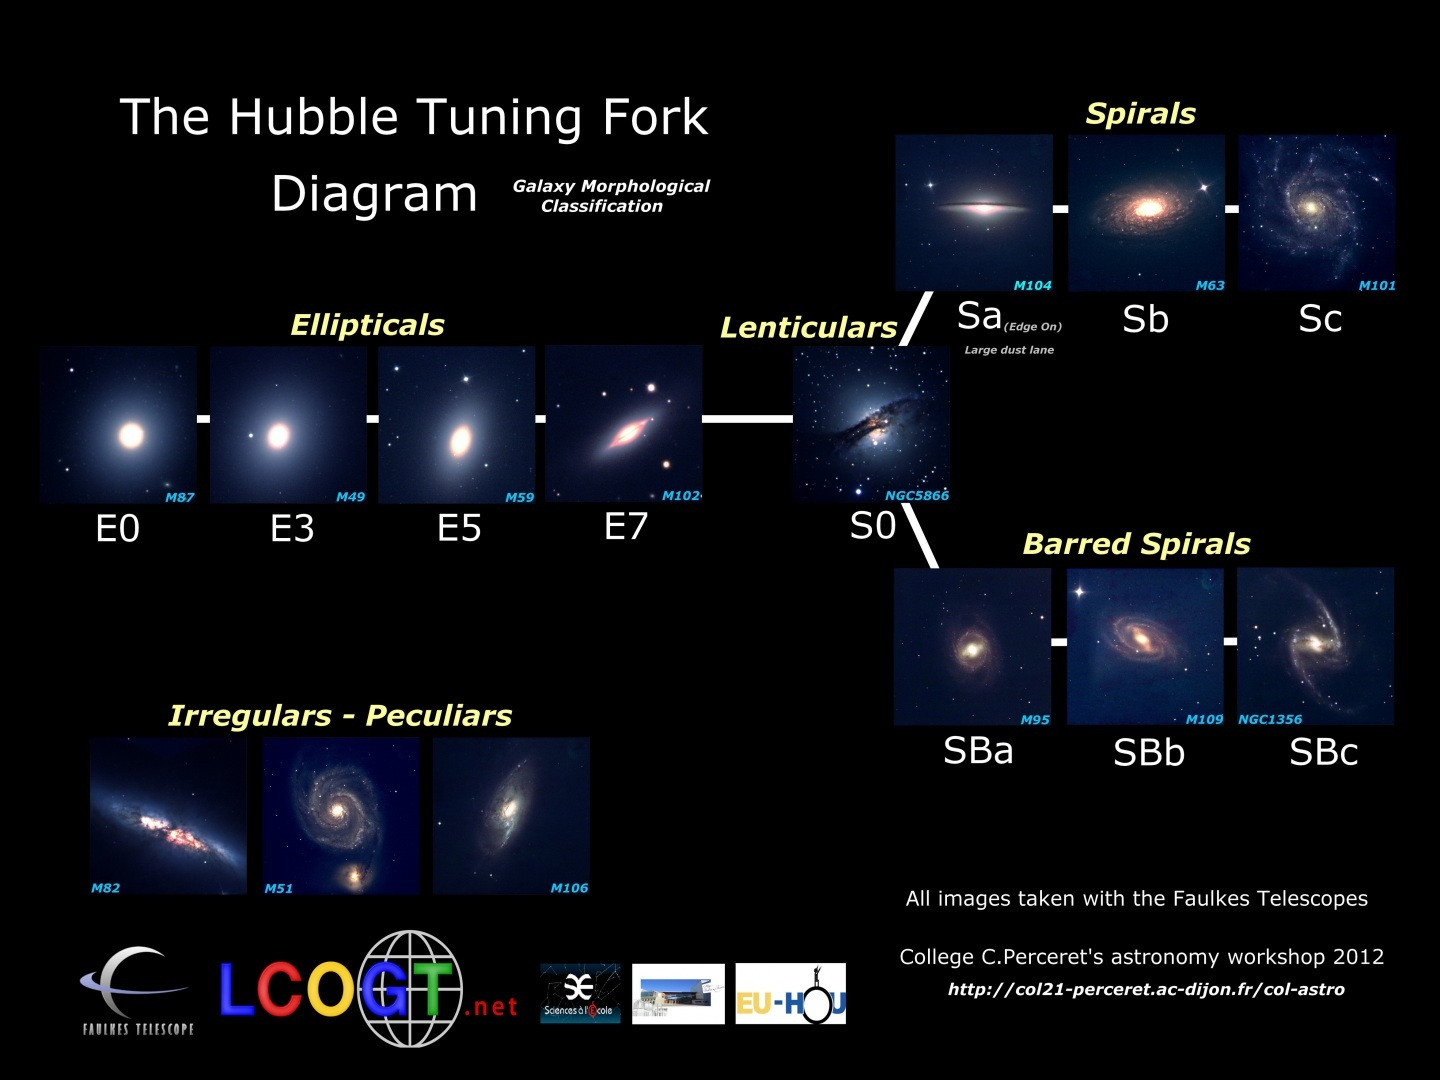
\includegraphics[width=\textwidth]{introduction/hubble-tuning-fork-diagram}
\caption{The Hubble sequence demonstrated graphically as the Hubble Tuning Fork (from \citealt{hubble_tuning_fork}). This diagram illustrates the Hubble classification of galaxies by their morphologies into ellipticals, spirals, lenticulars, and irregulars.}
\label{fig:hubble_tuning_fork}
\end{figure*}

Subsequent identification schemes would refine and build on the Hubble sequence as larger datasets became more readily available. These would contain a greater variety of extra-galactic objects and allow for arguments such as expanding the spiral category due to the importance of rings and lenses as their defining features \citep{1959HDP....53..275D}. 

Through Hubble's work, galaxies are comprehensively classified by their morphologies, however these do not fully reflect the internal content of a galaxy. For an indicator of the inner dynamics, fundamental parameters should be employed in tandem with the morphological classification. 

\vspace{2ex} % head space
\subsection{Dynamical studies of galaxies along the Hubble sequence}
\subsubsection{Angular momentum and the evolution of galactic dynamics}
\noindent
The mass, energy, and angular momentum are three physical values which are used as a quantitative classification of a galaxy. 

The angular momentum is of particular interest as the defining morphologies of a galaxy is most likely a result of the primeval mass--angular momentum distribution \citep{1970ApJ...160..831S}. The acquisition of this angular momentum in a protogalactic system was proposed by \cite{1969ApJ...155..393P} to be a result of the tidal interactions with nearby protogalaxies. Within a young spiral system, these tidal torques induce galactic spin and lead to massive extended haloes if spiral discs have radii comparable to present day observations. By extension, the dynamics of these discs and their stellar populations are modelled to demonstrate that their observed sizes and rotation velocities are consistent with the conservation of early angular momentum \citep{1998MNRAS.295..319M, 1997ApJ...482..659D}. 

Measurements of galactic specific angular momentum allows for the derivation of empirical relations between the stellar component of the angular momentum $j_*$ and mass $M_*$. These relationships can then be applied to describe the collective dynamics of galaxies \citep{fall1983}. If kinematic tracers are employed to measure $j_*$ and $M_*$ for large numbers of early-types (ellipticals and lenticulars) and late-types (spirals), then a plot such as Figure \ref{fig:romanowsky_fall_2012} reflects their dynamics by utilising independent variables and conservable physical quantities. The figure shows that both early and late types follow similar parallel trends which indicates an underlying connection between the physical parameters for galaxies. 

\begin{figure}
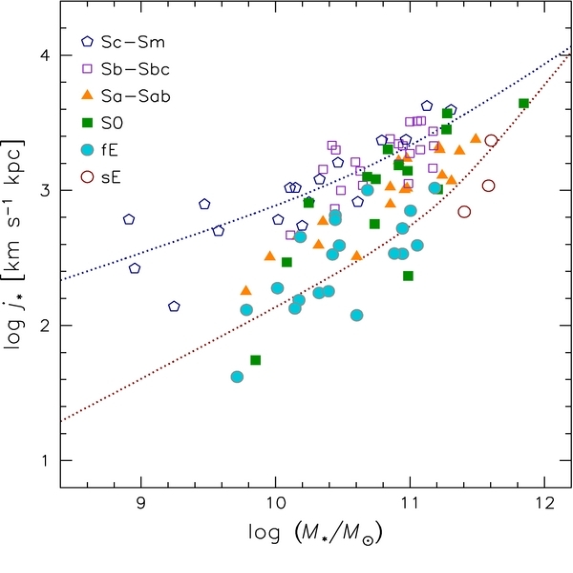
\includegraphics[width=1.0\linewidth]{introduction/romanowsky_2012_fig_3}
\caption{The total intrinsic specific angular momentum $j_*$ against total stellar mass $m_*$ for different galaxies (from \citealt{2012ApJS..203...17R}). Legend in upper left shows the galaxy types used. Ellipticals follow a similar relationship to spirals but with an offset of $\sim6$. This diagram represents one of the scaling relations for galaxies which reflect their internal dynamics.}
\label{fig:romanowsky_fall_2012}
\end{figure}

This coupling between $j_*$--$m_*$ represents one of the \textit{scaling relations} for galaxies. The importance of this particular relationship arises as it provides a fundamental scaling relation diagnostic for all galaxy types \citep{2012ApJS..203...17R}. With no full explanation available yet for the galaxy morphologies found in Hubble's sequence, scaling relations provide an opportunity to understand the fundamental dynamics which may lead to a comprehensive model of galactic formation and evolution.

\vspace{2ex} % head space
\subsubsection{Faber--Jackson and Tully--Fisher relations}
\noindent
Despite the pairing between angular momentum and mass for various galaxy types (spirals, and ellipticals) as shown in \cite{2012ApJS..203...17R}, scaling relations can be derived specifically for ellipticals and for spirals which would be better suited to describe their own specific properties within them.  

\begin{figure}
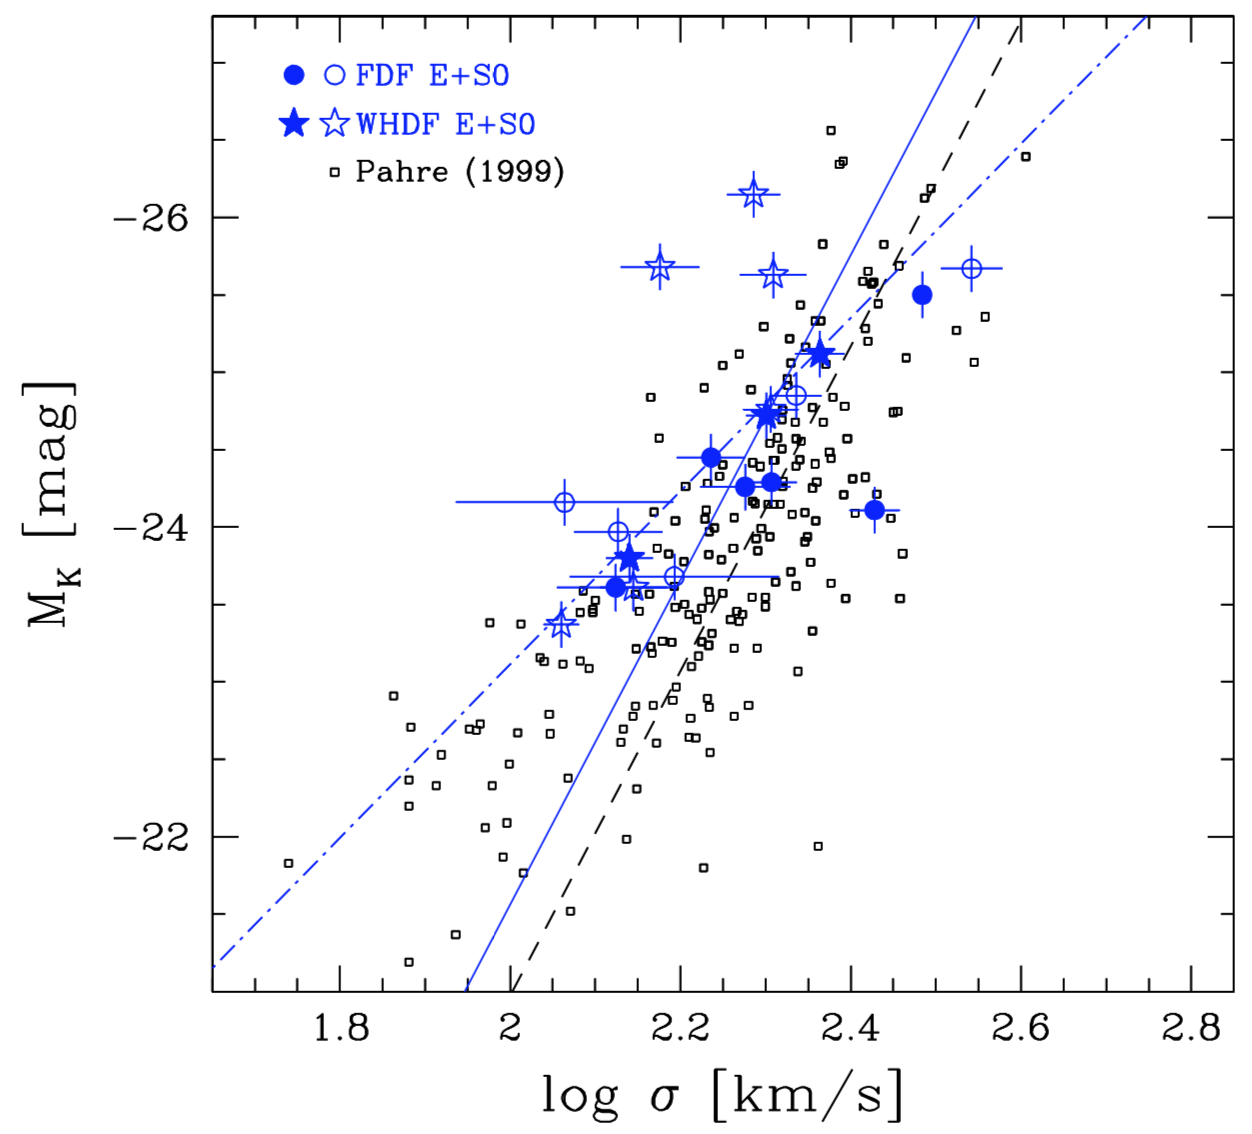
\includegraphics[width=\linewidth]{introduction/fritz_2009}
\caption{Faber--Jackson relation for early-type galaxies (from \citealt{2009MNRAS.393.1467F}). Data contains elliptical galaxies from FORS Deep Field and the William Herschel Deep Field samples. The FJR relates the luminosity $M_K$ with the velocity dispersion $\sigma$.}
\label{fig:faber_jackson}
\end{figure}

For ellipticals, \cite{1976ApJ...204..668F} produced a scaling relation between galaxy luminosity and velocity dispersions. The latter variable was chosen because through the virial theorem, the mass of galaxies can be estimated. With the availability of larger datasets, plots such as Figure \ref{fig:faber_jackson} illustrates the steady relationship between the luminosity and velocity dispersion. Through a well modelled Faber--Jackson relation, one potential use is to assess and understand galactic stellar populations and their evolutions \citep{2009MNRAS.393.1467F}, an important component in galaxy modelling.

\begin{figure}
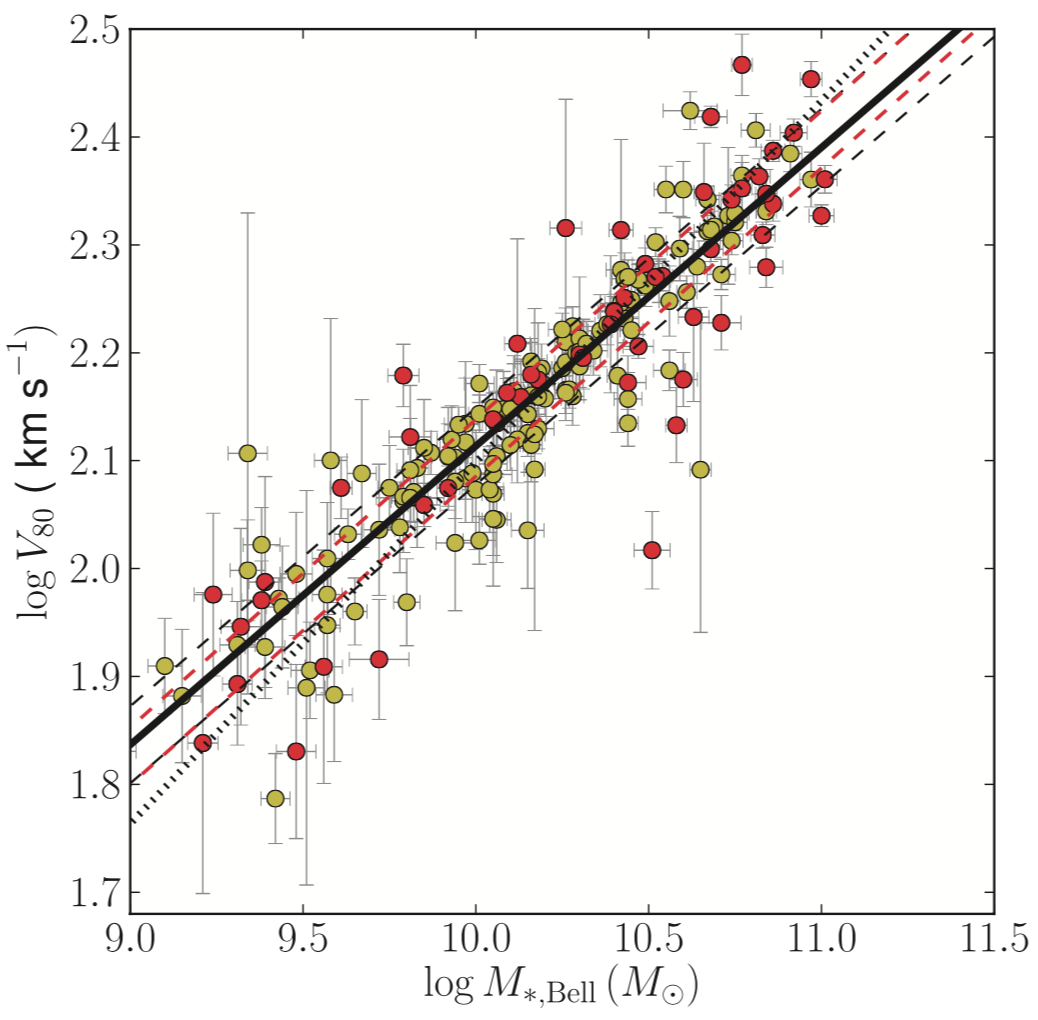
\includegraphics[width=\linewidth]{introduction/reyes_2011}
\caption{Tully--Fisher relation (TFR) for spiral galaxies (from \citealt{2012ApJS..203...17R}). The TFR relates galaxy stellar mass $M_*$ to the rotational velocity $V$.}
\label{fig:tully_fisher}
\end{figure}

On the other hand, \cite{1977A&A....54..661T} derived a relation between the absolute magnitudes and H$\alpha$ emission line widths for spiral galaxies. Another form re-expresses this to couple the stellar mass and rotational velocity of a galaxy. Figure \ref{fig:tully_fisher} demonstrates that there is a consistent relationship between these two parameters. In the production of this plot, \cite{2011MNRAS.417.2347R} would calibrate several Tully--Fisher models to consider the contributions from galactic discs, stars, and dark matter. Through these calibrations, the Tully--Fisher relation, like the Faber--Jackson can be applied to the construction of galaxy formation and evolution models.

Both Faber--Jackson and Tully--Fisher relations (FJR and TFR) quantify the physical properties of observable galaxies. It would be natural to question whether they are applicable to galaxies at higher redshifts ($z>0.3$) as these relations are calibrated with $z\sim0$ galaxy samples. For local galaxies, their dynamics are measured using various tracers (stars, gas, and neutral hydrogen). Comparatively, galaxy dynamics at high redshifts can only be quantified from bright emission lines, which produces a subjective view of galaxy dynamics. This partial bias is also found with the Hubble sequence where Hubble used local galactic objects as they provided the highest optical resolution to discern the different morphological features. 

One potential method to demonstrate whether local scaling relations are applicable at high redshifts is through simulating galaxies at various stages of evolution with galaxy formation models. 

\vspace{2ex} % head space
\subsection{Galaxy formation models}
\noindent
To produce a model which accurately describes the formation and evolution of galaxies, several physical processes must be accounted for. The main processes included in galaxy formation models are \citep{2015ARA&A..53...51S}: gravity, star formation, hydrodynamics and thermal evolution, black hole formation and growth, star formation feedback, active galactic nucleus feedback, stellar populations and chemical evolution, and radiative transfer. 

These processes interact and influence baryonic matter with the goal to create a dynamical galactic system. However, simulating these processes proves to be a challenge as there is difficulty in developing numerical algorithms which are able to accurately model their effects in a computationally efficient manner \citep{2015MNRAS.450.1937C}. Nonetheless, imperfect models are available for the component processes which simulate key observables and results. 

By analysing gravity, stellar formation, and hydrodynamic processes, a condensed overview of galaxy formation can be produced. If these models are shown to be accurate then locally--calibrated scaling relations could be tested using models of high--redshift galaxies.

\vspace{2ex} % head space
\subsubsection{Gravity}
\noindent
For the underlying building blocks to be present for galaxy creation, gravity must be at hand to drive cosmic structure formation. 

Employing cosmological models such as the $\Lambda$ cold dark matter model ($\Lambda$CDM), early conditions in the Universe can be simulated to demonstrate how gravity can induce dark matter clustering \citep{1978MNRAS.183..341W} and the condensation of dark matter halos \citep{1996ApJ...462..563N} to produce galaxies. Having an understanding of the distribution of dark matter halos in space is important in galaxy formation models as they reflect the overall distribution of mass.

As a result of the dark matter halos being dynamical objects, their gravitational interactions produce dynamical friction. This in turn can lead to the orbits of the galaxies within the halos to decay and eventually generate merger events. This transforms the structure and morphology of galaxies, and triggers additional star formation. 

\vspace{2ex} % head space
\subsubsection{Stellar formation}
\noindent
With initial stellar formation in protogalaxies, the key concept to model is how gas evolves into stars. Observations show that dense, molecular clouds within the interstellar medium (ISM) collapse to become stellar birthing grounds. One of the ways to simulate the converging gas is through numerical modelling \citep{1992ApJ...391..502K}, for example, assigning a \cite{1959ApJ...129..243S} stellar formation rate (SFR) law to the gas. However, as with galactic formation modelling, the inclusion of additional physical processes (such as magnetic fields and turbulence effects) produces systems which are highly nonlinear and multidimensional \citep{2007ARA&A..45..565M} thus more capable alternative methods are needed.

\cite{1996MNRAS.283.1388M, 1998ApJ...498..106M} developed a physically motivated set of tools to reconstruct stellar formation. They employed integrated galaxy emission properties to trace the evolution of galaxy luminosity density as a function of redshift. As a quantified result, Figure \ref{fig:madau} presents the ``Madau plot'' where SFRs are plotted against redshift for an epoch spanning from the present day to $z\approx8$. Within their research they utilised galaxy observational data in the UV and IR to directly measure the SFR and subsequently constrained the initial mass function (IMF) of stars.

\begin{figure}
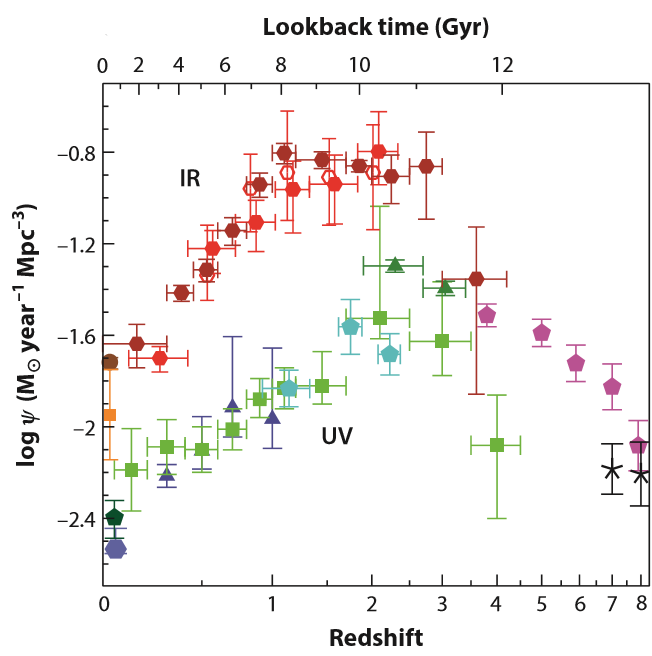
\includegraphics[width=\linewidth]{introduction/madau_2012}
\caption{Stellar formation rate (SFR) densities against redshifts (from \citealt{2014ARA&A..52..415M}). The SFR history of the Universe is shown in the IR and UV for a period between the present day and $z\approx8$.}
\label{fig:madau}
\end{figure}

However, these methods do not provide the capability to model complex galaxy formation, instead, hydrodynamic simulations must be considered. 

\vspace{2ex} % head space
\subsubsection{Hydrodynamics}
\noindent
Hydrodynamical modelling of galactic gas physics is the solving and evolution of hydrodynamic equations in a chosen gravity scheme. The \textit{Evolution and Assembly of GaLaxies and their Environments} (EAGLE) project implemented these equations to produce large scale N-body cosmological simulations \citep{2015MNRAS.446..521S}.

Using a $\Lambda$CDM universe, regions ranging in volume from 25 to 100 comoving Mpc were generated using numerical techniques and sub-grid models. They compared their EAGLE data with observations of the low-redshift universe to conclude that the simulation is generally able to replicate known observables. These include reproducing the galactic stellar mass function, disc galaxy sizes, and importantly producing agreement with the Tully--Fisher relation.

\begin{figure}
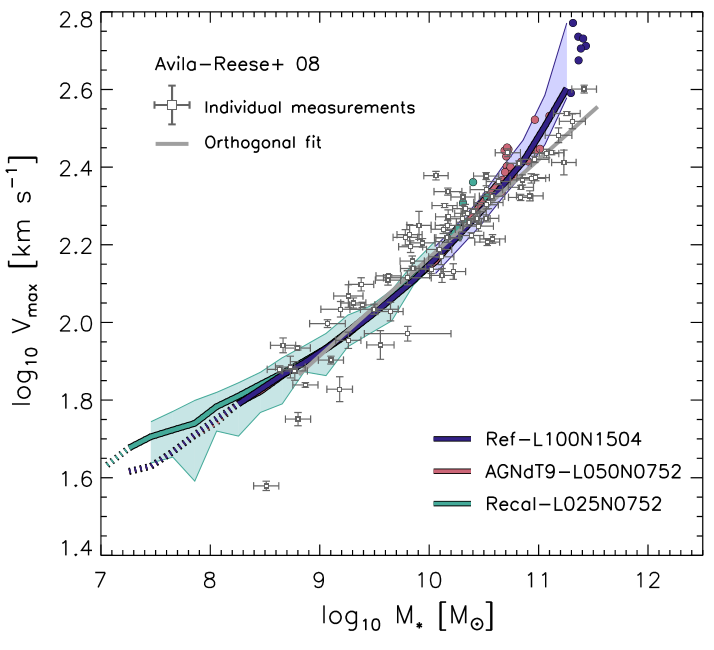
\includegraphics[width=\linewidth]{introduction/eagle_tully_fisher}
\caption{The Tully--Fisher relation (TFR) for spiral galaxies modelled with cosmological simulations (from \citealt{2015MNRAS.446..521S}). In this work the TFR is expressed as the relation between maximum rotation curve velocity $V_{\max}$ and stellar mass $M_*$. The legend in the lower right shows which simulated data was used, and the scatter points represent observational data.}
\label{fig:eagle_tully_fisher}
\end{figure}

Figure \ref{fig:eagle_tully_fisher} demonstrates that the EAGLE predictions are in remarkable agreement with the observational data. Cosmological simulations could therefore be an extremely useful tool in studying whether scaling relations evolve across cosmic history. These simulations have yet to be produced which offers a key opportunity to produce preliminary studies by utilising observational high--redshift galaxy data.

\vspace{2ex} % head space
\subsection{The Hubble Ultra Deep Field}
\noindent
In designing an experiment to test the applicability of scaling relations at high--redshifts, if data cannot be synthetically produced then it must be collected through observations.

\vspace{2ex} % head space
\subsubsection{HST}
\noindent
Optical data is the first out of two data--types required for a high--redshift analysis of scaling relations. One of the main constraints imposed on choosing a galaxy sample is the requirement for objects to be beyond redshift $z\approx0$. The \textit{Hubble Space Telescope} (\textit{HST}) has produced such data in the form of deep observational surveys.

The Hubble Deep Field (HDF) was one such survey. The expectation of HDF was to aid in resolving problems within studies of galaxy formation \citep{1996AJ....112.1335W}. Before HDF, observations of distant galaxies were limited by observational depth. The Canada-France Redshift Survey \citep{1995ApJ...455..108L} observed galaxies with redshifts $0.5<z<1.2$ in $B$ and $I$-photometric bans. They determined that the central surface brightness of the disks in their spiral sample was more than 1.2 mag brighter than objects at $z\approx0$, pus their $B$-band images appeared to be less regular than when observed at longer wavelengths. However, they did conclude that the observed galaxy morphologies at their redshift range were similar to those seen locally.

The HDF survey would utilise \textit{HST}'s ability to resolve and image galaxy systems out to high redshifts. Data was collected for a four arcmin$^2$ field over an exposure period of 0.5 million s using Wide-Field Planetary Camera 2 (WFPC2) on \textit{HST}. Four specific filters (F300W, F450W, F606W, and F814W) were chosen to try and balance image depth, colour information, and restrict the scattered light from Earth. The final reduced sample would contain 3000 galactic objects with a large number at $z>1$. \cite{1998ApJ...496L..93D} is one study which utilised the HDF sample to demonstrate that galaxy populations for high redshifts is markedly different than those at present times. For example, the $z>2$ epoch appeared to contain a higher number of spiral and irregular galaxies which was attributed to the occurrence of more galaxy merger events.

To extend measurements to the period of recombination from $z\sim6-10$ to $z\sim1100$ required changes either in the observational method or with the observational instrument. The first observations of this epoch were made using the Sloan Digital Sky Survey through the detection of the Gunn-Peterson hydrogen edge in the spectra of distant quasars \citep{2001AJ....122.2850B,2002AJ....123.1247F}.

For an optical survey to observe large numbers galaxies at these redshifts, the luminosity function inferred from the HDF suggested that data should be collected for a wider area but to a lesser depth than HDF. The Great Observatories Origins Deep Survey (GOODS; \citealt{2004ApJ...600L..93G}) performed such a survey with the optical component achieved by \textit{HST}. Four filter bands (F435W, F606W, F775W, and F850L) were again used, but instead of WFPC2, the Advanced Camera for Surveys (ACS) was employed in it's place. From an observed area 30 times larger but 1 mag shallower than HDF, a sample of 60,000 galaxies was produced. Analysis of this data when coupled with K20 spectroscopic information would support the predominance of spirals and irregulars in $0.5<z<1.5$ galaxy samples \citep{2005MNRAS.357..903C}.

It was evident that with the success of deep surveys such as HDF and GOODS, naturally, an ultradeep survey would be commissioned to perform deeper galaxy formation studies, this was the Hubble Ultra Deep Field (HUDF). One of several goals for this project was to extend information on galaxies at the intermediate-redshift range $2<z<5$ and attempt to observe the reionisation boundary at $z\sim6$ \citep{2006AJ....132.1729B}. The specifications of the data collection and data reduction for one version of the HUDF will be further discussed in Section \ref{sec:obs_hst}.

An estimate of the number of galaxies at different redshifts was performed by assuming the galaxy luminosity distributions follow a Schechter function \citep{1976ApJ...203..297S}. Ranging from $1<z<7$ and with a magnitude limit between 28 and 29, a rough non-corrected value of 72700 sources was estimated to be observed in the HUDF. In reality, refined analysis and object detection algorithms such as SEXtractor \citep{1996A&AS..117..393B} reduced this estimation to $\sim10000$ objects, nonetheless, this is still an immense number of galaxies. 

\begin{figure*}
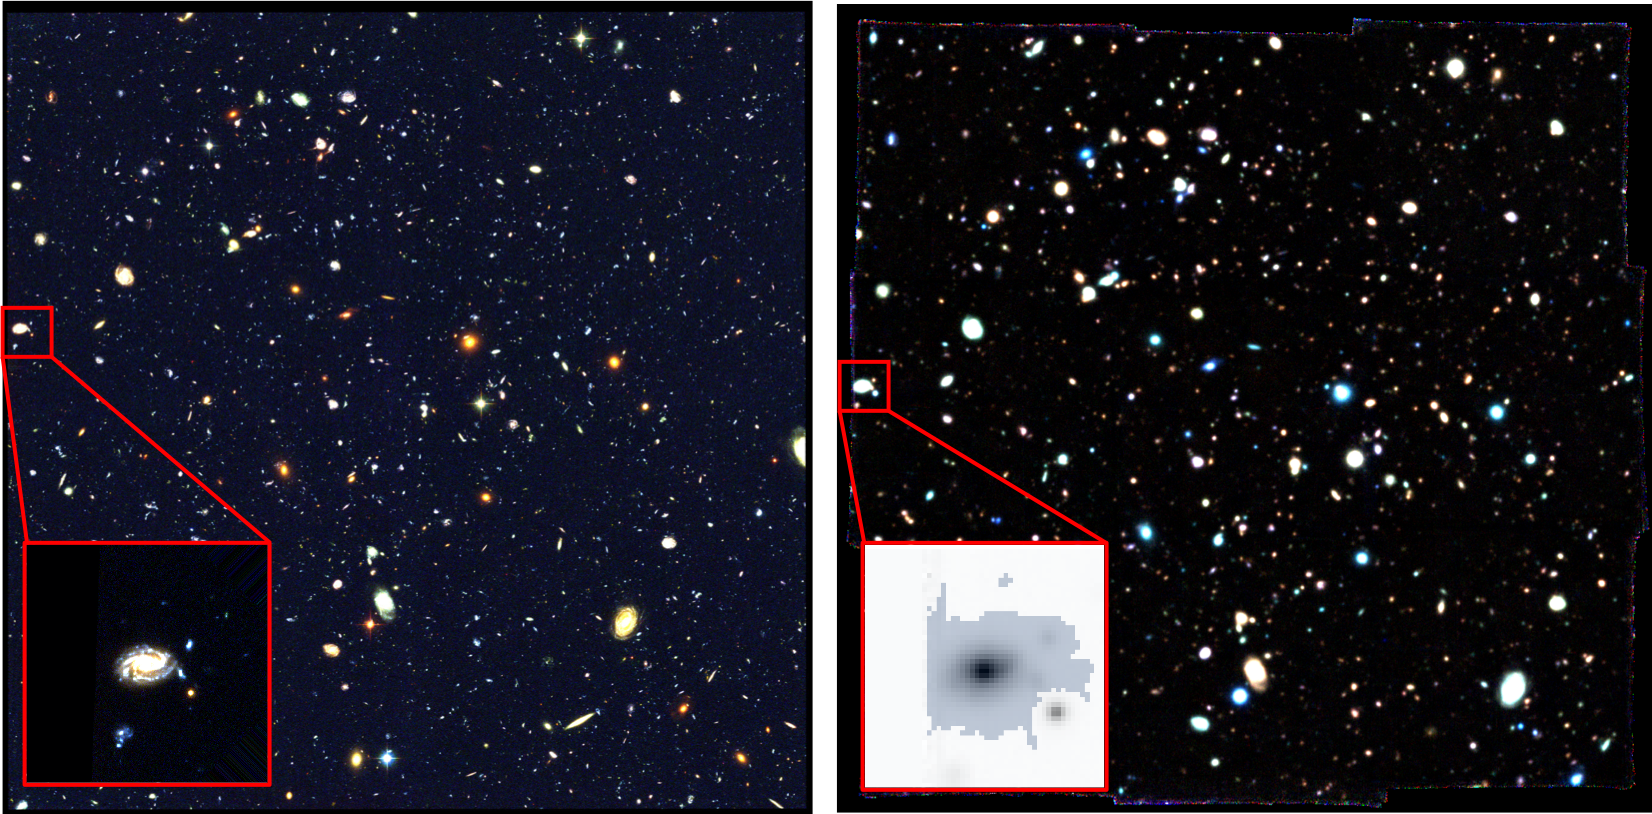
\includegraphics[width=\textwidth]{introduction/hudf_frame.pdf}
\caption[Hubble Ultra Deep Field]{\textit{Left-hand panel}: colour composite image at an image scale of 30 mas for the HUDF from \textit{HST} ACS/WFC, Hubble eXtreme Deep Field project data \citep{2013ApJS..209....6I}. Frames in three filter bands (F775W, F606W, and F435W) were combined to represent the RGB channels within a colour image. \textit{Right-hand panel}: colour image of the MUSE HUDF region. The spectra wavelength range (4650 \AA--9300 \AA) of the MUSE cube was divided into three equal regions (4650 \AA--6180 \AA, 6180 \AA--7730 \AA, 7730 \AA -- 9300 \AA), collapsed, and then combined to create an RGB image. Highlighted in both images is object RAF-24420 \citep{2015AJ....150...31R}, the \textit{HST} data has a higher optical resolution whereas the MUSE data has the superior resolution in it's spectroscopic data.}
\label{fig:hst_muse_hdf}
\end{figure*}

The data retrieved for the HUDF would later be combined with survey data from other \textit{HST} projects (supernovae follow-up observations, HUDF09, CANDELS, and HUDF12) to produce the deepest image of the sky ever taken in the optical/near-IR, the eXtreme Deep Field (XDF; \citealt{2013ApJS..209....6I}). Figure \ref{fig:hst_muse_hdf} contains a collapsed colour image for the HUDF region made using XDF data. The data from filters F775W, F606W, and F435W were combined into an RGB colour image. Representative of the same area, the XDF strived to enhance and augment the original HUDF data to provide a deeper dataset. 

For studies of the early universe, the HUDF is a remarkable dataset. It provides high-resolution optical data for galaxies covering a wide range of redshifts which makes it highly suitable for studying changes in the characteristic luminosity, the evolution of morphologies, and the testing of locally-derived galaxy scaling relations.

\vspace{2ex} % head space
\subsubsection{MUSE}
\noindent
With optical data for high--redshift galaxies available in the form of the HUDF, testing scaling relations such as TFR and FJR additionally requires spectroscopic data to quantify redshifts, velocities and velocity dispersions.

It is generally known that calculating redshifts requires spectra of observed objects and for chemical elements or compounds, the value of which can be summarised as,
\begin{equation}
    z=\frac{\Delta \lambda}{\lambda_{\text{emit}}}=\frac{\lambda_{\text{obs}}-\lambda_{\text{emit}}}{\lambda_{\text{emit}}},
    \label{eqn:redshift}
\end{equation}

where $z$ is the dimensionless quantity redshift, $\lambda_{\text{emit}}$ is the emitted wavelength of an object, and $\lambda_{\text{obs}}$ is the observed wavelength of an object \citep{1933AcHPh...6..110Z}.

The application of redshifts to extra-galactic astronomy has it's origins with \cite{1913LowOB...2...56S} who studied the radial velocities for the Andromeda galaxy. By attaching a spectrograph to a telescope, they were able to collect spectrograms for Andromeda and derive it's velocity with the Doppler approximation $z\approx v/c$. Slipher used the shifted spectral lines to calculate a mean velocity of $\Minus$300 km $s^{-1}$ and noted how this value for a spiral galaxy was much higher than the velocities stars. They had observed the effects of redshift on the spectra of galaxies, and arrived at the result that Andromeda is travelling towards us. Subsequent work \citep{1914LowOB...2...66S} would also demonstrate the rotational motion of spiral galaxies. Through observing NGC 4594 with a spectrograph across the long axis of the galaxy, they obtained spectra with lines analogous to those produced by the diurnal rotation of a planet. Through the use of spectroscopy, Slipher was therefore able to establish the kinematic dynamics of galaxies. 

Additional information can be obtained from galaxy spectra through measuring the widths of spectral lines. Also known as velocity dispersions, these widths encode a variety of knowledge related to the internal makeup of the galaxy. Measurements of the velocity dispersions for elliptical galaxies can be used to derive the galaxy masses with the virial theorem \citep{1958BOTT....2q...8P} and be used as an observational constraint on galaxy formation theories \citep{1964ApJ...139..284F}.

Alternatively, the velocity dispersions can be used to quantify the kinematics of stars and gas within the galaxies. The general method used: the stellar kinematics can be measured from the widths of the absorption lines in a galaxy spectra, and the gas kinematics properties from specific emission lines. \cite{2001A&A...374..394V} provides one example of this method for a sample of 20 nearby disc galaxies. They quantified stellar and gas velocities ($V_*$, $V_g$) and velocity dispersions ($\sigma_*$, $\sigma_g$) for integrated galaxy spectra to produce $\sigma_g$ versus $\sigma_*$ plots, and they then identified the dynamics across the galaxy's kinematic axis to produce rotation curves and velocity dispersion plots. 

A spectra obtained for a galaxy therefore encodes vast amounts of information relating to it's properties and dynamics. These derived values reflect and provide an insight into the formation and evolution of galaxies. 

The star formation within a galaxy can be expressed with two particular functions \citep{1979ApJS...41..513M}: the spatially averaged rate of galaxy star formation (the stellar birthrate) and the frequency distribution of stellar masses at birth (the initial mass function, or IMF). The latter relationship is of particular interest as it allows for the derivation of the evolution, surface brightness, chemical enrichment, and baryonic content of galaxies \citep{2003PASP..115..763C}. Originally defined by \cite{1955ApJ...121..161S}, the IMF cannot be determined directly through observations, instead it can be indirectly constrained through methods such as using spectra absorption lines \citep{2012ApJ...760...70V}.

\begin{table}
\begin{center}
\begin{tabular}{c@{\hskip 20pt}c} 
 \hline
 \textbf{Type} & \textbf{Colour and notable lines} \\ [0.5ex] 
 \textit{O} & Hot blue-white (HeII, HeI) \\
 \textit{B} & Hot blue-white (HeI, HI ) \\
 \textit{A} & White (Balmer, CaII) \\
 \textit{F} & Yellow-white (CaII, FeI, Cr,I) \\
 \textit{G} & Yellow (CaII, FeI,  \\
  & neutral metals) \\
 \textit{K} & Cool orange (CaII H and \\ 
  & K, metals) \\
 \textit{M} & Cool red (TiO, VO, neutral \\
  & metals) \\
 \textit{L} & Very cool, dark red, infrared \\
  & (Molecular absorption, CrH, \\
  & FeH, H$_2$O, CO, Na, K, Rb, Cs) \\
 \textit{T} & Coolest, infrared (CH$_4$, CO) \\
 \hline
\end{tabular}
\caption{The Harvard Spectral Classification for stellar objects \citep{1916AnHar..76...19C}. Stars are defined by their colour (temperature) and features seen from their spectra \citep{stellar_colour, 1925PhDT.........1P}. Provided are spectral types, and their associated colour plus the main emission or absorption lines. Figure \ref{fig:spectral_types} provides examples of the possible observed spectra for spectral types \textit{OBAFGKM}.}
\label{table:spectral_classification}
\end{center}
\end{table}

Once obtained, the IMF provides an estimate of the present-day and initial stellar and brown dwarf populations of a galaxy. Knowledge of the IMF utilised with integrated galaxy spectra allows for the stellar types contained within the galaxy to be predicted.

\begin{figure}
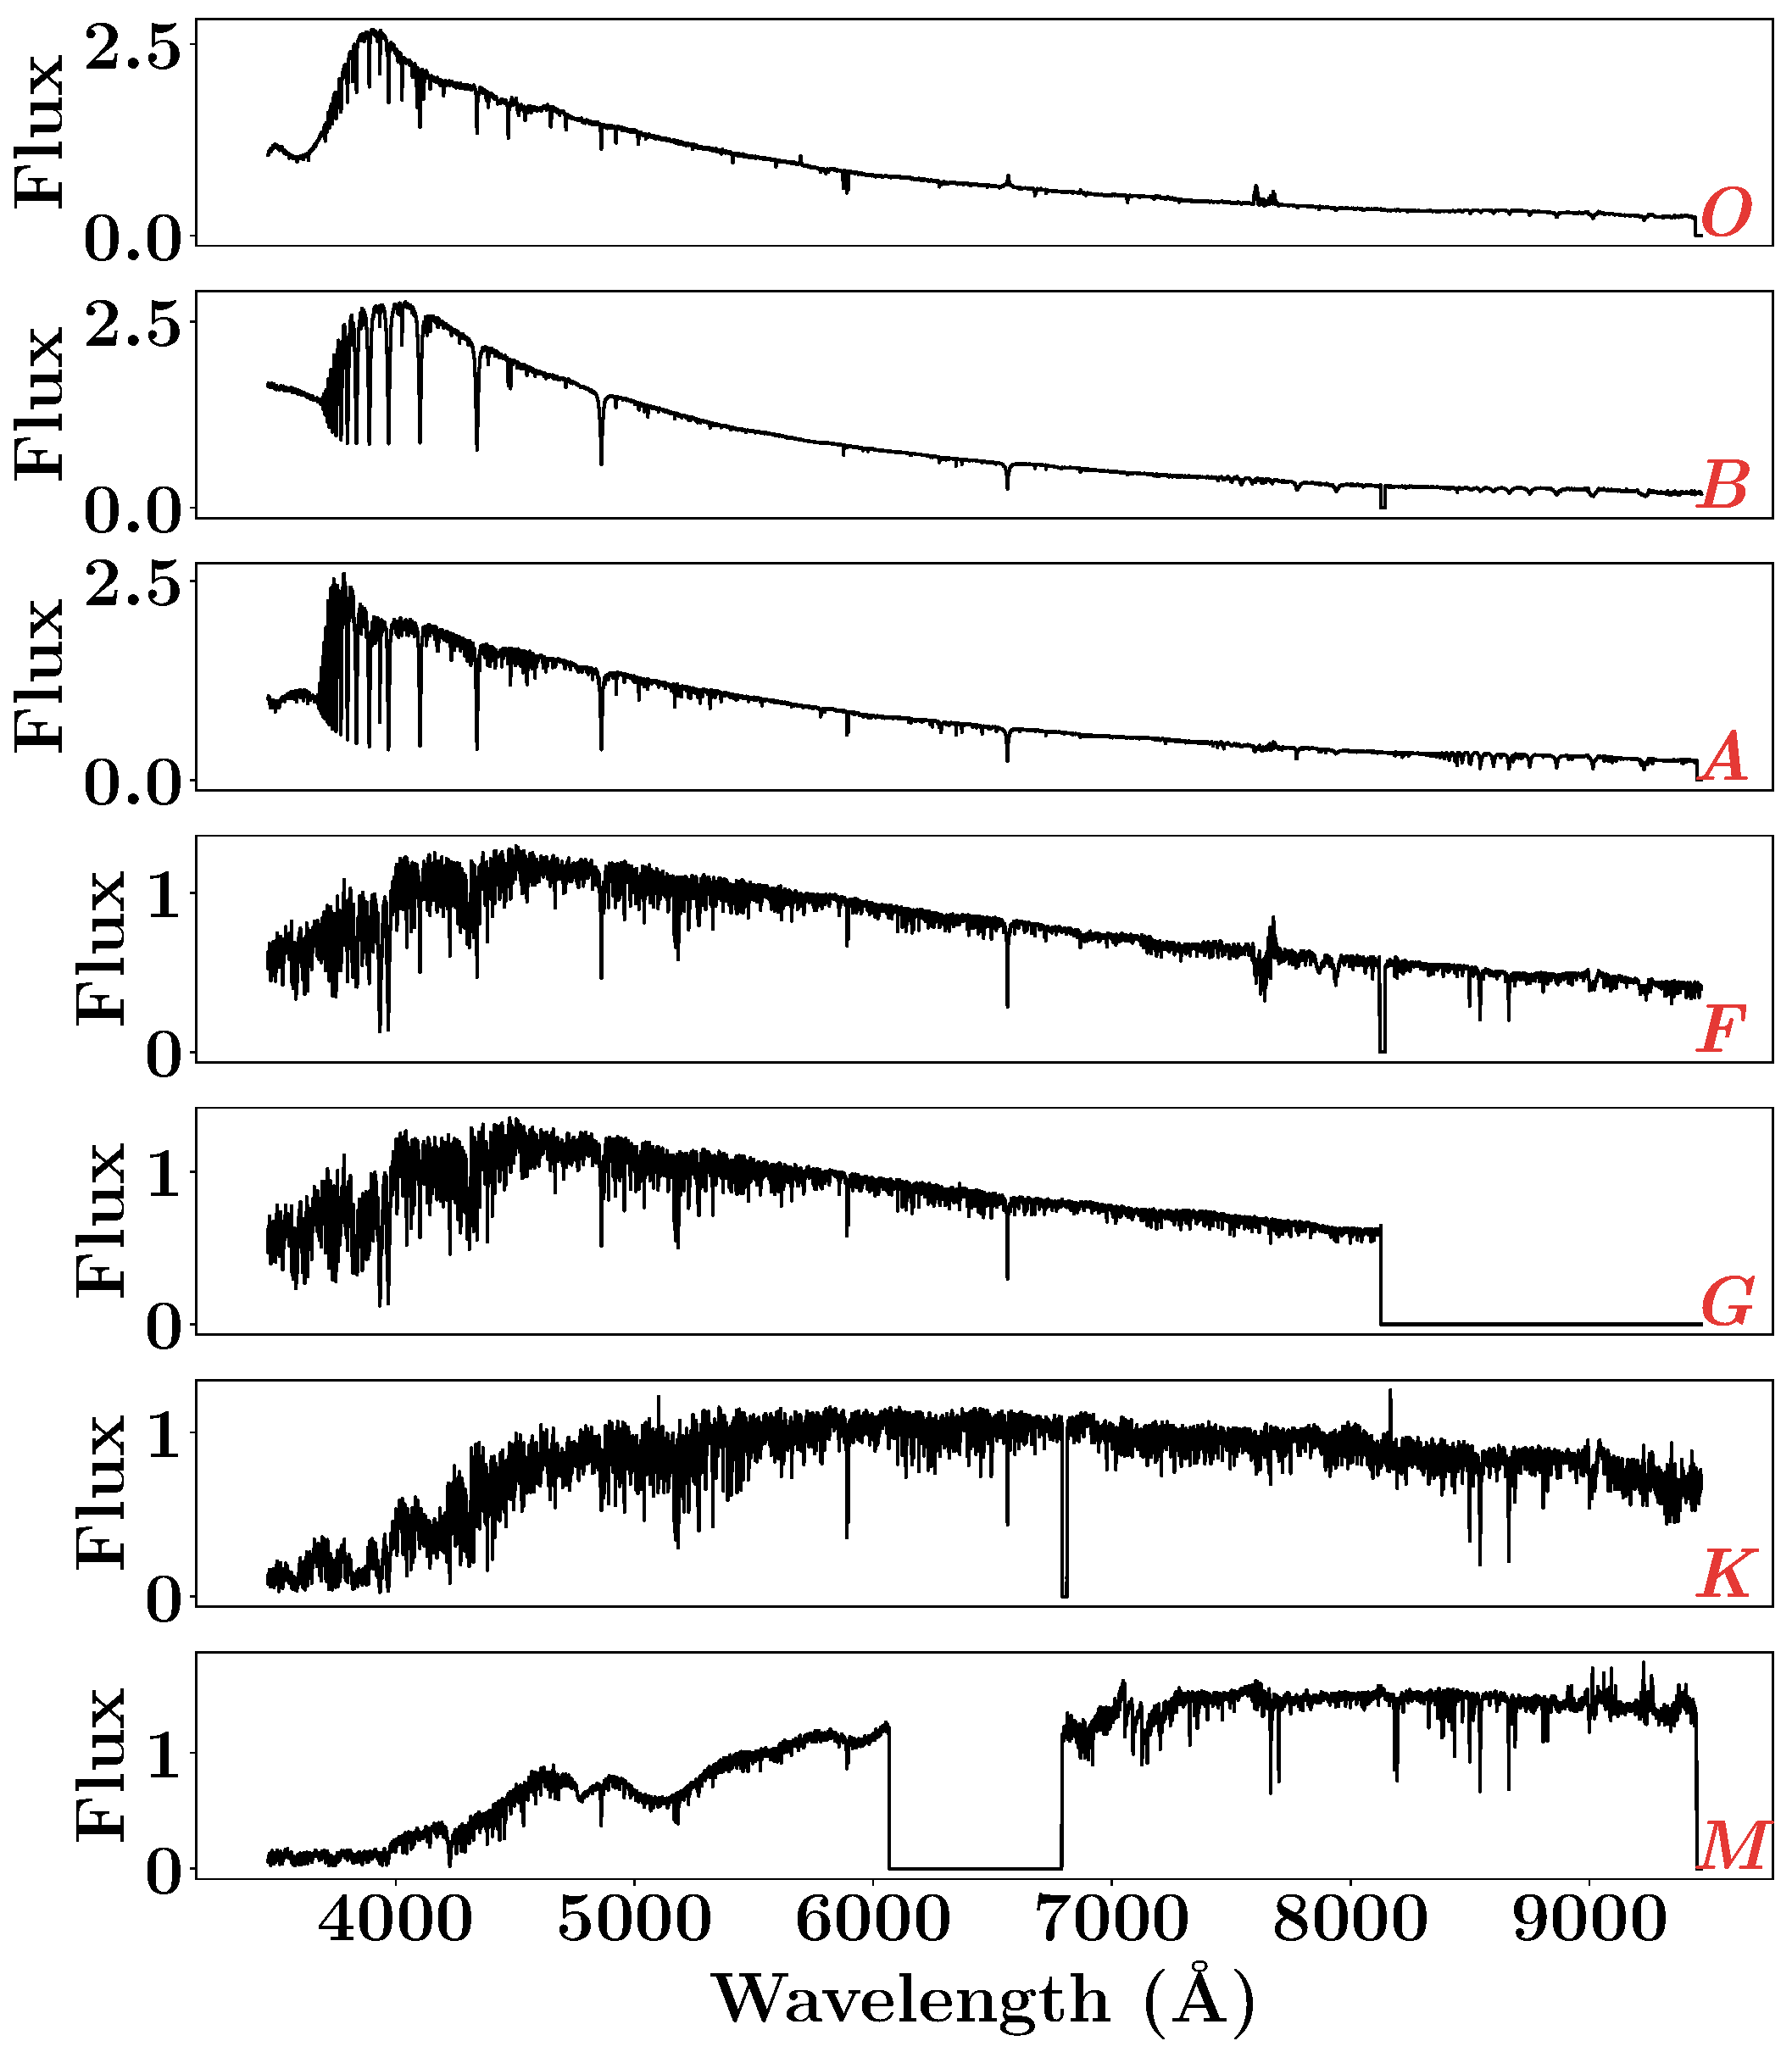
\includegraphics[width=1.0\linewidth]{introduction/spectral_types}
\caption{Example spectra for spectral types \textit{OBAFGKM}. Taken from the Indo-US Library of Coudé Feed Stellar Spectra \citep{2004ApJS..152..251V}, the stars used have metallicities [Fe/H]$_{\odot} \approx0$  and IDs: 30614 (\textit{O}), 17081 (\textit{B}), 39866 (\textit{A}), 5015 (\textit{F}), G 7-6 (\textit{G}), 5858 (\textit{K}), and G 176-11 (\textit{M}). These spectra demonstrate that older types (\textit{FGKM}) have larger amounts of absorption and emission lines when compared to younger types (\textit{OBA}) as they have spent a greater amount of time undergoing nuclear fusion. Galaxy spectra will contain combinations of these stars which produces a unique profile.}
\label{fig:spectral_types}
\end{figure}

An extrapolation can be performed as each star contains an individual spectral signature due to the elemental composition of the stellar atmospheres. Stars can be classified by absorption and emission lines and by optical colour to produce the Harvard Spectral Classification. Table \ref{table:spectral_classification} provides a summary of this classification scheme and Figure \ref{fig:spectral_types} contains examples of observed spectra for individual stellar types. 

An alternative way to classify stars is through their metallicities. Denoted as $Z$ or [Fe/H], the metallicity is the measure of a star's chemical abundance and can be found as the ratio between iron-to-hydrogen with respect to the Sun \citep{1976ARA&A..14...43A}. The Sun is defined as [Fe/H]$_{\odot} \equiv 0$. \cite{1944ApJ...100..137B} introduced stellar population groups which utilises metallicity: Population I are metal rich stars [Fe/H]$>-1$  found in discs, and Population II are metal poor stars [Fe/H]$<-1$ found in galaxy halos. A third group, Population III, has been theorised as stars which contain little to no metals [Fe/H]$<-3$ \citep{1981ApJ...248..606B}. Spectroscopy can once again be utilised to calculate [Fe/H] for Population I and II \citep{2004A&A...415.1153S}, Population III stars have yet to be observed but next-generation instruments such as ULTIMATE-Subaru provide the potential to do so \citep{2019arXiv190301613M}

From the dynamics and kinematics of the stars and gas within the galaxy to calculating the stellar population, a wealth of information is obtainable from galaxy spectra. It is therefore unsurprising that spectroscopic data should be collected for high--redshift galaxies as there is no particular reason why the physics of the spectra would change. Coupled with optical data, the locally-derived scaling relations can then be tested and verified. 

The Multi-Unit Spectroscopic Explorer (MUSE) on the Very Large Telescope (VLT) is one of the few current instruments which is able to provide spectroscopic data for redshifts $z>6$ \citep{2010SPIE.7735E..08B}. The key dataset obtained by MUSE which allows for the testing of the scaling relations is the MUSE Hubble Ultra Deep Field \citep{2017A&A...608A...1B}. Specifics on the data collection and data reduction will be discussed in Section \ref{sec:obs_muse}. 

Though MUSE's capability of integral field spectroscopy, deep spectroscopic observations were performed on the Hubble field to produce the MUSE HUDF which covers 90\% of the original HUDF. Containing a wavelength range of 4650 {\AA} to 9300 {\AA}, the data for the MUSE HUDF can be collapsed into three regions (4650 \AA--6180 \AA, 6180 \AA--7730 \AA, 7730 \AA -- 9300 \AA) to produce an RGB colour image (Figure \ref{fig:hst_muse_hdf}). When compared to the HST HUDF, the MUSE field appears to have much lower optical resolution, however, this comparison is partly null as the primary use of the MUSE data is for spectroscopic analysis.

\vspace{2ex} % head space
\subsection{Project study and aims}
\noindent
With optical and spectroscopic data available for a large sample of high--redshift galaxies in the HUDF, this project seeks to understand whether locally-derived scaling relations are applicable to the high--redshift universe.

The paper is organised as follows. In Section \ref{sec:observations} the observations and data reduction techniques will be described for the HST and MUSE HUDFs, and then the methodology provided for the construction of the galaxy sample used in this study. Section \ref{sec:discussion} presents the emission and absorption line modelling for the high--redshift galaxy spectra to obtain velocity dispersion and radial velocity values, the gas and stellar kinematics will be compared, the Voronoi tessellation work to test the Tully--Fisher and Faber--Jackson relations presented, the applicability of the scaling relations summarised and compared, and then a discussion of potential future studies. Finally, the conclusions will be presented in Section \ref{sec:conclusions}.

Cosmological quantities calculated in this study assumed a flat Universe with $H_0=70$ km s$^{-1}$ Mpc$^{-1}$, $\Omega_m=0.3$, and $\Omega_\Lambda=0.7$.

\vspace{2ex} % head space
\section{Observations and data reduction} \label{sec:observations}
\subsection{HST XDF HUDF} \label{sec:obs_hst}
\noindent
Optical images of galaxy morphologies were obtained from a colour composite HUDF frame created with publicly released XDF data\footnote{Available from: \href{http://xdf.ucolick.org}{http://xdf.ucolick.org}.}. 

\begin{figure}
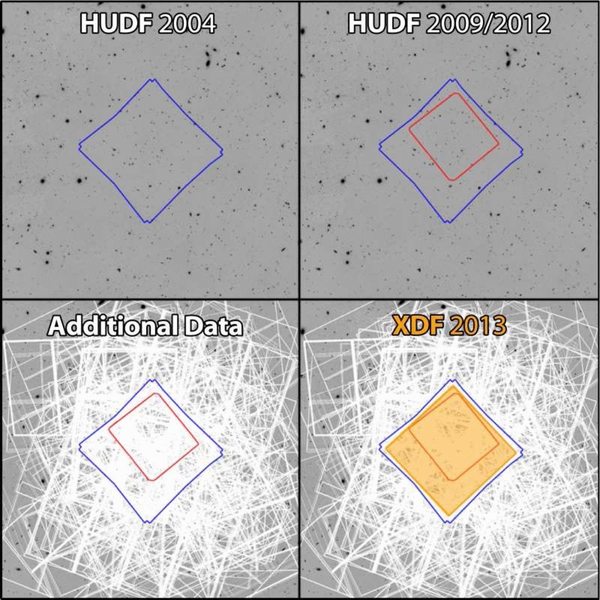
\includegraphics[width=\linewidth]{introduction/xdf_frame.jpg}
\caption[Hubble eXtreme Deep Field]{The production of the XDF (from \cite{2013ApJS..209....6I}). Upper left frame shows the original optical HUDF (blue) from ACS which contributed $50\%$ of the XDF data set. Upper right shows the introduction of the HUDF09 IR data (red) from WFC3/IR, forming $20\%$ of XDF. Lower left shows the final $30\%$ contribution from 17 other \textit{HST} programs (white) of which the large majority came from CANDELS ACS and WFC3/IR data, and the HUDF12 WFC3/IR data. Lower right shows the final produced XDF frame (orange).}
\label{fig:xdf_frame}
\end{figure}

\vspace{2ex} % head space
\subsubsection{XDF data and data reduction}
\noindent
Original imaging of the HUDF \citep{2006AJ....132.1729B} employed the ACS Wide Field Camera (ACS/WFC) instrument on \textit{HST} in four optical filter bands: F435W, F606W, F775W, and F850LP. The observations were obtained in 400 orbits between September 2003 and January 2004. Subsequent \textit{HST} programs would re-image the region in optical and IR bands to further deepen the data available for the field. The XDF project combines all available data for the HUDF region from the period July 2002--December 2012 which were taken with ACS/WFC and \textit{HST} Wide-Field Camera 3 Infra-Red (WFC3/IR) to produce the deepest ever field \citep{2013ApJS..209....6I}. Figure \ref{fig:xdf_frame} shows the production of the XDF with the data from 20 \textit{HST} programs.

For the ACS/WFC optical component, a field of 10.8 arcmin$^2$ was produced to a depth of $30.8(5\sigma)$ AB mag in a $0.35''$ aperture. 1972 exposures in five filter bands was utilised: 164 exposures for F435W, 286 exposures for F606W, 460 exposures for F775W, 362 exposures for F814W, and 700 exposures for F850LP. The XDF field is centred on coordinates RA$=03^{\text{h}} 32^{\text{m}}38.5^\text{s}$ and Dec.$=\Minus 27 \degree 47 ' 00.0''$ (J2000). The ACS/WFC channel includes two $4096 \times 2048$ pixel detectors at a scale of $0.05''$ pixel$^{-1}$ to supply a $202'' \times 202''$ effective field of view. 

As described by \cite{2013ApJS..209....6I}, observations were chosen from the MAST \textit{HST} archive for ACS/WFC by searching a 13 arcminute radius around the original HUDF coordinates ($\alpha=03^{\text{h}} 32^{\text{m}}39.0^\text{s}$, $\delta=\Minus 27 \degree 47 ' 29.0''$), and limiting the search to HST filters F435W, F606W, F775W, F814W, and F850LP, and exposure time to $>100$ s. 

The optical images in the XDF dataset were processed with the ACS calibration pipeline \texttt{calacs} (2012.2). This process subtracts bias, corrects for dark current, masks bad pixels, and performs flat-fielding. For images taken after \textit{HST} Servicing Mission 4, they were corrected for charge transfer efficiency degradation \citep{2010PASP..122.1035A}, bias shift, bias striping \citep{2010hstc.workE..54G}, and amplifier crosstalk \citep{2010hstc.workE..55S}. 

The data production pipeline applied to each filter dataset was \texttt{APSIS} \citep{2003ASPC..295..257B}. Similar to the software package \texttt{MultiDrizzle} \citep{2003hstc.conf.....A}, each image was passed through a drizzle--blot--drizzle cycle. Drizzling, or Variable-Pixel Linear Reconstruction, is a method where the resolution of undersampled images can be improved by using a shift-and-add technique and interlacing \citep{2002PASP..114..144F}. To blot is to map a median image onto the input plane of individual images, accounting for image shifts and geometric distortion. 

Images would be background-subtracted and drizzled onto a tangential plane pixel grid. They would then be median-stacked and blotted back to each input image position and used as a template for cosmic-ray injection. A cosmic-ray mask would be generated for each image and combined with a data quality array. A final image mosaic would be produced by drizzling input images onto a single mosaic and combined with inverse-variance weight maps which considers all noise sources (readout, dark current, and background noise). 

The world coordinate system of each image was refined to produce precise registration across all ACS/WFC images because the pointing accuracy of \textit{HST} is only good to within a few arcseconds. An image registration process was ran with \texttt{superalign} \citep{2013ApJS..209....6I} where positions of a source were taken from a reference catalogue and from catalogues generated for each image, an accurate shift and rotation correction would then be calculated and applied to the input image. The reference catalogue was generated from combining the original HUDF F775W image with an astrometrically calibrated GOODS mosaic to provide accurate alignment for within and outside the HUDF area.

The final data produced would be a frame representing each filter band for ACS/WFC: F435W, F606W, F775W, F814W, and F850LP.

\vspace{2ex} % head space
\subsubsection{Coloured HUDF}
\noindent
To produce the colour image of the HUDF, the dataframes for F435W, F606W, and F775W were selected from the XDF dataset and combined into an RGB image using a \texttt{Python} routine. The filters correspond to the $I$-, $V$-, and $B$-bands, therefore they were used to approximately represent the B, G, and R channels within a colour image. The final coloured field can be seen in Figure \ref{fig:hst_muse_hdf}.

\vspace{2ex} % head space
\subsection{MUSE HUDF} \label{sec:obs_muse}
\noindent
Primary analysis in this paper was performed on spectroscopic data for the HUDF from the MUSE HUDF Survey\footnote{Available from: \href{http://muse-vlt.eu/}{http://muse-vlt.eu/}.}.

\vspace{2ex} % head space
\subsubsection{MUSE data and data reduction}
\noindent
Observations of the HUDF were performed with MUSE in Wide Field Mode on the VLT under the guarantee time observing ESO programs. Over the period September 2014--February 2016, 137 h of telescope time was used to used to cover the HUDF with a mosaic of nine MUSE fields (UDF-01 through UDF-09). Each MUSE field has the same area as the detector field of view, $1\times1$ arcmin$^2$. The instrument has a spectral range of 4650--9300 {\AA}, a spatial resolution of 0.2 arcsec, and a spectral resolution of $R\sim3000$. Figure \ref{fig:muse_frame} presents the locations and orientations of the MUSE fields over the HUDF.

\begin{figure}
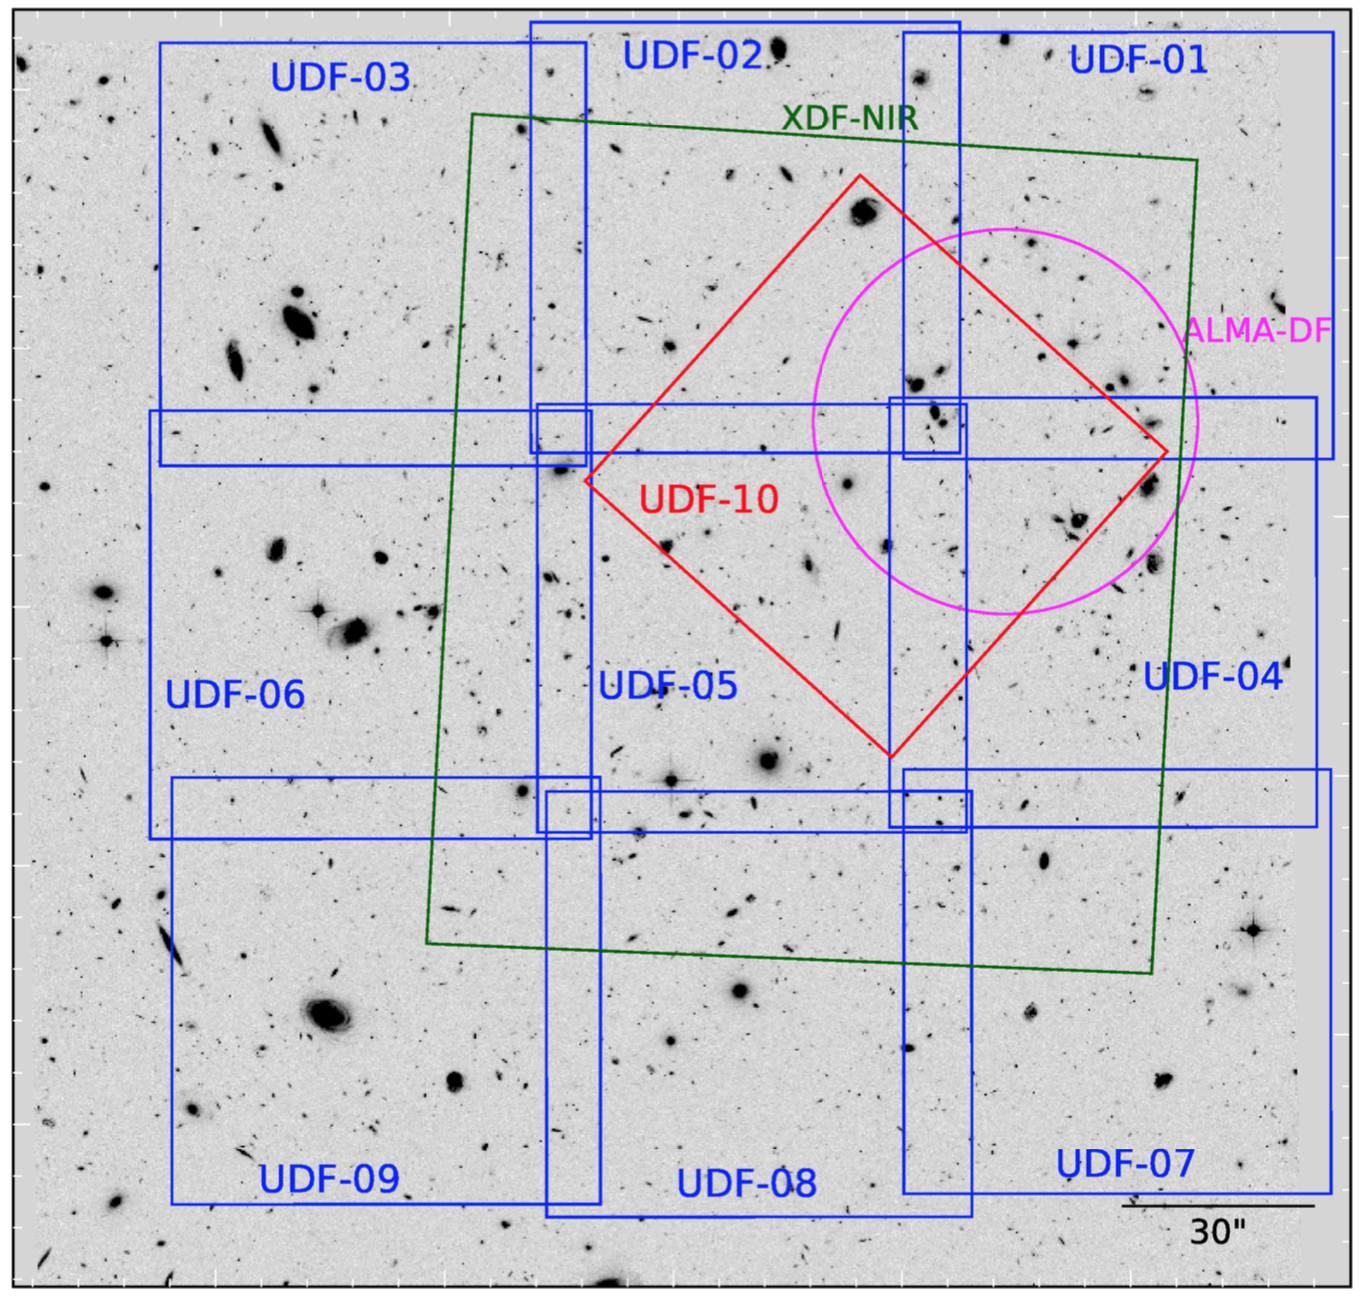
\includegraphics[width=\linewidth]{introduction/muse_frame}
\caption[MUSE HUDF]{MUSE fields taken of the HUDF (from \cite{2017A&A...608A...1B}). The field region and orientation of the final \texttt{mosaic} (UDF01--09, blue) has been overlaid on the HST ACS F775W image. The UDF10 fields (red), XDF near-IR field (green), and ALMA deep field from the ASPECS pilot program (magenta, \citealt{2016ApJ...833...67W}) are additionally marked.}
\label{fig:muse_frame}
\end{figure}

A total of 227 exposures were taken, each had an integration time of 25 minutes to limit the entry into the sky-noise-limited regime and to limit the impact of cosmic rays. The final \texttt{mosaic} of the HUDF achieved a depth of $\approx10$ h over an area of 9.92 arcmin$^2$ ($90\%$ of the original HUDF) within an approximate region of $3.15'\times3.15'$. 

An additional deeper observation was taken, UDF-10, over the deepest region of the XDF near-IR data and to overlap as much as possible with the deep ALMA pointing from the ASPECS pilot program \citep{2016ApJ...833...67W}. UDF-10 covers an area of $1.15$ arcmin$^2$ and reaches a depth of 31 h.

As described by \cite{2017A&A...608A...1B}, the raw science data was reduced with the MUSE standard pipeline v1.7 dev. Individual exposures were processed by \texttt{scibasic} which employed daily calibrations (flatfields, bias, arc lamps, twilight exposures) and geometry table to produce a table containing all pixel information: location, wavelength, photon count, and an estimate of variance. Known bad pixels from CCD defects were masked. An illumination exposure was used to correct each exposure for flux variations at slice edges due to small temperature changes between morning calibrations and science exposures. The illumination exposures were chosen to be the ones nearest in temperature to the science frames.

The \texttt{scipost} pipeline would perform astrometric and flux calibrations on the table of pixel information. All flux calibration values obtained over all nights were scaled to the same mean level to remove transparency variations. The median of the stack was then obtained to produce the final reference response. A data cube would then be created with \texttt{makecube} using the default 3D drizzling interpolation process. 

A self-calibration procedure was applied to correct for detector instabilities and imperfect flatfielding. A standard mask would be applied to all bright objects within the data. The median flux of each thin mirror slice of the MUSE image slicer was calculated for a bin of wavelength range 200-300 {\AA}. The individual slices flux were offset to the mean of all slices and channels over same wavelength bin. Outliers would be rejected by using a $15\sigma$ clipping based on the median absolute deviation.

Inter-stack defects (dark or bright regions) at the edges of each slice stack for deep exposures of empty fields were additionally corrected for. An optimum mask was produced by median-combining all exposures onto an instrumental grid based on pixel coordinates, the locations of defects were identified to produce a bad pixel table. The 3D drizzle algorithm would introduce additional interpolation effects, so a 3D mask was produced for the cube by running the pipelines with and without the bad pixel table. 

Individual masks were produced and applied for specific defects such as Earth satellite trails or anomalous high dark levels or bias residuals. 

The recentered and self-calibrated pixel table of each exposure would be sky subtracted with \texttt{ZAP} \citep{2016MNRAS.458.3210S}, and datacubes created on a fixed grid. A world coordinate system was pre-defined for the full mosaic region and frames UDF01--09 were projected onto the grid. 

Variance and exposure properties for the datacubes would be subsequently calculated and derived as detailed by \cite{2017A&A...608A...1B}. 

The 227 datacubes of the \texttt{mosaic} would be combined using estimated flux corrections from a reference \textit{HST} image. A $5\sigma$-clipping based on median absolute deviation estimates would be used to remove outliers, then an average performed on all volume sampling elements (voxels; $0.2''\times0.2''\times1.25$ \AA). The corrected variance was propagated and an exposure map datacube produced. The final science datacube has a median depth of $9.6$ h and contains $(n_x, n_y, n_z)=947\times 945\times 3681=3.29 \times 10^9$ voxels. The cube has three axes: two tangential representing the field-of-view (arbitrarily defining them as $x$ and $y$), and one extending perpendicular which contains the spectroscopic information ($z$). 

In addition to the final data frame, a catalogue of 1574 objects was produced for both UDF10 and \texttt{mosaic} fields \citep{2017A&A...608A...2I}\footnote{Available from VizieR with keyword \texttt{J/A$\Plus$A/608/A2}: \href{http://vizier.u-strasbg.fr/viz-bin/VizieR}{http://vizier.u-strasbg.fr/viz-bin/VizieR}.}. This catalogue contains derived spectroscopic redshifts using the MUSE data, magnitudes found in several HST filters, and the flux values for various spectra emission peaks. The sources were extracted using a combination of the UVUDF catalogue \citep{2015AJ....150...31R} and directly from the MUSE cube with the methodology described in \cite{2017A&A...608A...1B, 2017A&A...608A...2I}.  

\vspace{2ex} % head space
\subsection{Production of galaxy sample}
\noindent
To produce the sample of galaxies used in this study, source extraction was performed on the MUSE datacube. The data was firstly collapsed into a single 2D frame by taking the median spectroscopic value along each voxel.

Source detection was then applied with the Starlink implementation (2018A; \citealt{2014ASPC..485..391C}) of the \texttt{SExtractor} package \citep{1996A&AS..117..393B}. Parameters were chosen to deblend galaxies, obtain their positions, and produce good signal-to-noise (S/N) values. The minimum number of connected pixels to register a detection was set to 5, no detection filter was specified, the zero-point in the photometry was set to 0.0, and the image scale set to match MUSE, 0.2 arcsec pixel$^{-1}$. A symmetric correction mask was chosen to account for overlapping objects, this mask replaced the overlap with counterparts symmetric to the objects’ centre. The FWHM seeing was set to 0.8 arcsec, and the size of the background mesh was set to 128. 

\begin{figure}
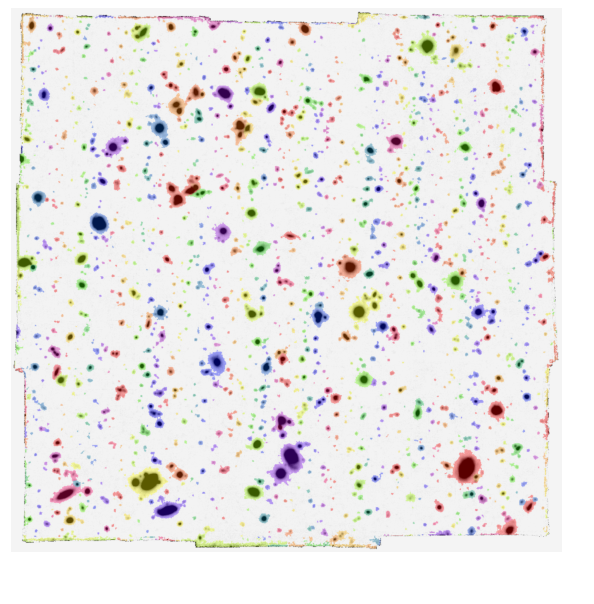
\includegraphics[width=\linewidth]{data/muse_seg_map.pdf}
\caption[MUSE Segmented]{Galaxy segmentation map overlaid on collapsed 2D MUSE HUDF field. Segmentation map was created by the \texttt{SExtractor} object extraction routine, and each coloured area defines an individual object.}
\label{fig:muse_seg_map}
\end{figure}

Using these parameters, 1823 objects would be detected from the collapsed MUSE frame. The exported catalogue from the extractor routine contains: object ID, $x$ and $y$ positions, the flux and associated error for the detected object, the RA and Dec., the semi-minor $a$ and semi-major $b$ axis values, the rotation of the object with respect to the horizontal, and a probability that the object is a star. 

Alongside this catalogue a segmentation map was produced in tandem. Figure \ref{fig:muse_seg_map} shows this map superimposed onto the collapsed 2D MUSE field. Each galaxy during the extraction routine had a region and a unique ID defined for it, the segmentation map summarises this information into a single frame and allows for individual object masks to be produced to isolate the spectroscopic data for a specific galaxy. This would be particularly useful if two objects happened to overlap. 

The \texttt{SExtractor} and MUSE catalogues were then combined so that the HST and redshift data would be accessible along with the extracted information. Employing Starlink's TOPCAT software \citep{2005ASPC..347...29T}, the celestial coordinates in both catalogues were compared and matched using a sky algorithm within a maximum error of $1.0''$. This would produce a combined catalogue to contain 837 objects.

For the purpose of the investigation into the applicability of local scaling relations, this sample was further reduced so only high S/N and high--redshift galaxies would remain. 

The catalogue was first sorted by the MUSE spectroscopic redshifts and it was decided that 41 objects with $z<0.3$ were to be removed, leaving 796 potential galaxies. This was defined because the project would use the bright [OII]$\lambda\lambda$3726,29 {\AA} emission doublet to measure the dynamics of the gas and through considerations of the MUSE working spectral range beginning at 4650 {\AA}, Equation \ref{eqn:redshift} was employed with $\lambda_{\text{obs}}=4800$ {\AA} and $\lambda_{\text{emit}}=3727$ {\AA} to produce $z=0.3$. 

To enable analysis on a sample of just galaxies, the catalogue was organised by the \texttt{SExtractor} probability that the object is a star, and only objects with a probability less than 0.50 were chosen. This would further reduce the sample to 252 potential galaxy objects.

Each of these sources were individually extracted from the MUSE \texttt{mosaic} cube. A $50\times 50$ pixel$^2$ area was drawn around the central pixel coordinate of each object on the $xy$ field-of-view plane, the matching spectroscopic data along $z$ would be extracted, and the corresponding $xy$ segmentation map area obtained. 

With the 252 individual cubes, it had to be ensured that: the objects were in fact galaxies, an [OII] doublet feature could be found within the spectra, and enough S/N was present for the absorption lines to be modelled.  

By organising the objects by their V-band magnitude and through [OII] doublet modelling (further discussion in Section \ref{sec:disc_oii_modelling}), a magnitude limit of 25.0 mag was imposed on the sample. This was approximately the point where the fitting routine could recognise the [OII] doublet in the spectra and apply a model.

\begin{sidewaystable*}
\vspace{50ex}
%\centering
\begin{tabular}{c@{\hskip 10pt}c@{\hskip 10pt}c@{\hskip 10pt}c@{\hskip 10pt}c@{\hskip 10pt}c@{\hskip 10pt}c@{\hskip 10pt}c@{\hskip 10pt}c@{\hskip 10pt}c} 
 \hline
 \textbf{Cube ID} & \textbf{RAF ID} & \textbf{RA (deg)} & \textbf{Dec. (deg)} & \textbf{F606W mag.} & \textbf{$\boldsymbol{z}$} & \textbf{$\boldsymbol{V_*}$ (kms$^{-1}$)} & \textbf{$\boldsymbol{\sigma_*}$ (kms$^{-1}$)} & \textbf{$\boldsymbol{V_{OII}}$ (kms$^{-1}$)} & \textbf{$\boldsymbol{\sigma_{OII}}$ (kms$^{-1}$)} \\ [0.5ex] 
C1804 & 24420 & 53.1783773 & -27.76824447 & $21.4864(8)$ & $0.66850(6)$ & $153531(10)$ & $182(25)$ & $153471(24)$ & $ 147(35)$ \\ 

C1578 & 22735 & 53.13064889 & -27.79026088 & $21.880(1)$ & $0.66640(5)$ & $153185(7)$ & $117(12)$ & $153094(18)$ & $ 139(25)$ \\ 

C849 & 21651 & 53.17251203 & -27.79636076 & $22.125(1)$ & $0.347053(5)$ & $89414(8)$ & $3.8(7)$ & $89314(18)$ & $ 79(24)$ \\ 

C286 & 24587 & 53.16992265 & -27.77102451 & $21.1412(9)$ & $0.62169(1)$ & $145050(7)$ & $58(6)$ & $144939(17)$ & $ 91(16)$ \\ 

C5 & 20595 & 53.15639984 & -27.81081513 & $21.5823(8)$ & $0.66459(2)$ & $152807(9)$ & $78(10)$ & $152768(21)$ & $ 110(24)$ \\ 

C767 & 21364 & 53.18023505 & -27.79892259 & $21.958(1)$ & $0.6673(1)$ & $153328(10)$ & $148(21)$ & $153250(24)$ & $ 141(34)$ \\ 

C414 & 7253 & 53.15153909 & -27.76201929 & $22.546(3)$ & $0.42451(5)$ & $106177(10)$ & $106(21)$ & $106076(23)$ & $ 128(42)$ \\ 

C549 & 24515 & 53.15256871 & -27.76950996 & $22.858(3)$ & $0.33644(1)$ & $87049(9)$ & $25(6)$ & $86943(22)$ & $ 85(32)$ \\ 

C175 & 8246 & 53.18480046 & -27.77745246 & $23.570(4)$ & $0.52255(2)$ & $126111(11)$ & $127(25)$ & $126029(28)$ & $ 82(28)$ \\ 

C1129 & 9958 & 53.13928756 & -27.78066897 & $23.677(4)$ & $0.73403(2)$ & $165114(19)$ & $60(15)$ & $165020(46)$ & $ 95(41)$ \\ 

C765 & 23794 & 53.15817553 & -27.78109416 & $22.391(2)$ & $0.619373(2)$ & $144615(12)$ & $65(12)$ & $144512(30)$ & $ 64(20)$ \\ 

C1075 & 3630 & 53.16129898 & -27.79547518 & $23.720(3)$ & $0.30988(3)$ & $80989(11)$ & $143(41)$ & $80925(26)$ & $ 77(38)$ \\ 

C540 & 24348 & 53.16236468 & -27.77506443 & $21.4602(8)$ & $0.41894(2)$ & $105015(8)$ & $60(10)$ & $104899(19)$ & $ 91(25)$ \\ 

C895 & 39778 & 53.14168389 & -27.77310068 & $24.291(6)$ & $0.52461(2)$ & $126561(18)$ & $0.5(2)$ & $126434(43)$ & $ 73(38)$ \\ 

C554 & 38260 & 53.14916378 & -27.76363345 & $23.401(3)$ & $0.737184(4)$ & $165687(12)$ & $123(20)$ & $165565(30)$ & $ 70(19)$ \\

C109 & 9475 & 53.18591136 & -27.77561507 & $24.084(4)$ & $1.42553(8)$ & - & - & 265631(137) & 105(83) \\ 

C310 & 8531 & 53.16632928 & -27.76858816 & $23.778(5)$ & $1.29533(2)$ & - & - & 249090(83) & 75(39) \\ 

C363 & 8672 & 53.16395412 & -27.76905273 & $24.569(7)$ & $0.41891(3)$ & - & - & 104894(57) & 57(47) \\ 

C486 & 51705 & 53.18782913 & -27.79405589 & $20.6113(5)$ & $0.345393(8)$ & - & - & 88944(12) & 91(19) \\ 

C254 & 4686 & 53.19373778 & -27.78787018 & $24.572(7)$ & $0.43534(3)$ & - & - & 108346(44) & 48(30) \\ 

C759 & 8949 & 53.14617923 & -27.77103939 & $24.108(5)$ & $1.3155(2)$ & - & - & 251719(134) & 108(88) \\ 

C1394 & 2908 & 53.1525505 & -27.80037599 & $24.99(1)$ & $1.4254(1)$ & - & - & 265614(101) & 0.04(2) \\ 

C847 & 21703 & 53.17365111 & -27.7973635 & $24.218(5)$ & $0.66543(1)$ & - & - & 152920(28) & 34(10) \\ 

C1665 & 50714 & 53.15110943 & -27.80949195 & $24.552(4)$ & $1.08753(3)$ & - & - & 220642(99) & 79(54) \\ 

C541 & 24353 & 53.16081556 & -27.77537746 & $22.442(2)$ & $0.62149(6)$ & - & - & 144902(21) & 111(25) \\ 
 \hline
\end{tabular}
\caption{Parameters for the final reduced sample of 35 galaxies. Columns show the galaxy ID, the ID from the UVUDF Catalogue \citep{2015AJ....150...31R} (RAF ID), the object right ascension (RA) and declination (Dec.), the magnitude of the object in the HST F606W filter, the calculated galaxy redshift ($z$), the galaxy stellar velocity ($V_*$) and velocity dispersion ($\sigma_*$), and the galaxy [OII] gas velocity ($V_{OII}$) and velocity dispersion ($\sigma_{OII}$. Note that only 11 galaxies could be analysed for both gas and stellar components. The remaining 24 only their [OII] doublet, 15 of those galaxies are shown here with the remaining 9 contained in Appendix \ref{appendix:rest_of_final_sample}. The main analysis in this paper only used galaxies which contained kinematic results for both stellar and gas.}
\label{table:final_sample}
\end{sidewaystable*}

\begin{figure}
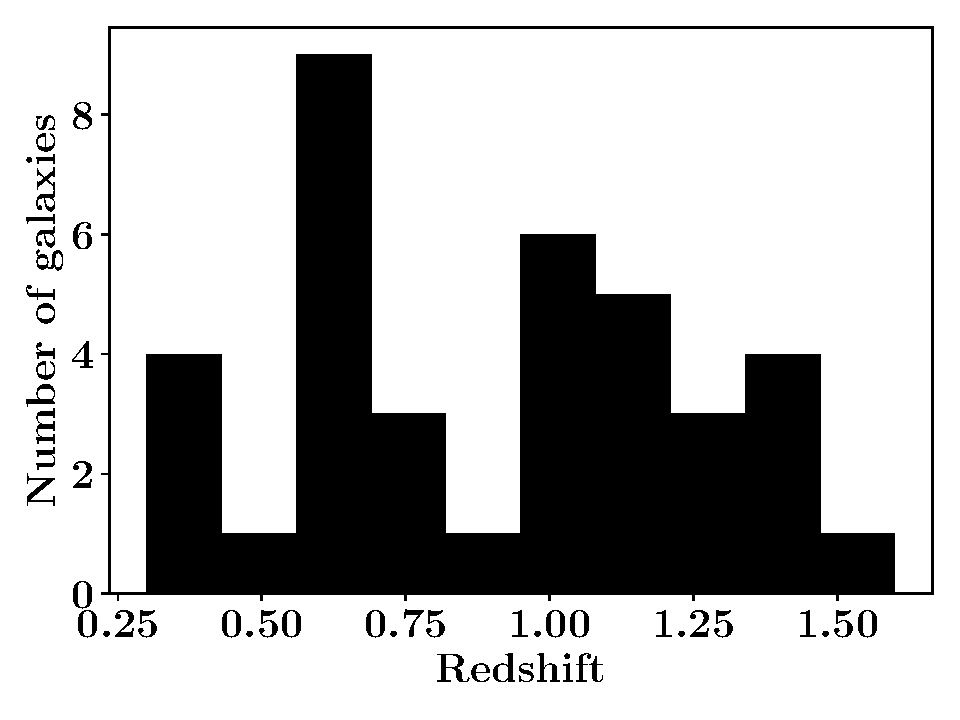
\includegraphics[width=\linewidth]{data/redshift_distribution_oii_emitters.pdf}
\caption{The redshift distribution of the final sample of 35 galaxies. Each bin represents a redshift width of 0.13. There are a large number of galaxies found at $z\sim0.6$, but the majority are spread across higher redshifts $z\gtrsim1.0$.}
\label{fig:redshift_dist}
\end{figure}

The remaining 75 sources were subsequently reduced to a final sample of 35 galaxies. The spectra for 40 of the objects were found to contain no particular [OII] feature which meant they could not be used for the later investigation. Table \ref{table:final_sample} and Table \ref{table:rest_of_final_sample} in Appendix \ref{appendix:rest_of_final_sample} provides catalogue data and results from later analysis of galaxy spectra for the 35 objects. Figure \ref{fig:redshift_dist} shows the distribution of the redshifts for the galaxies, a large number are at higher redshifts ($z\gtrsim1.0$) which make them key for testing the locally--derived scaling relations.  

\begin{figure*}
  \subfloat{\label{fig:image_sn_vband}%
  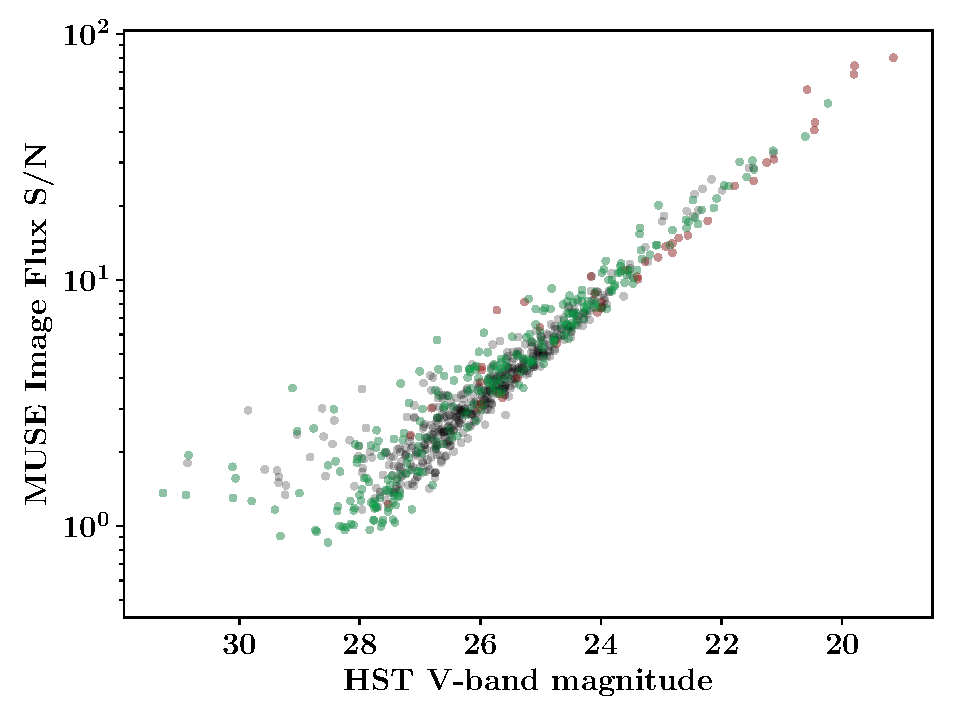
\includegraphics[width=0.5\textwidth]{data/image_sn_vs_vband}%
  }
  %
  \subfloat{\label{fig:spec_sn_vband}%
  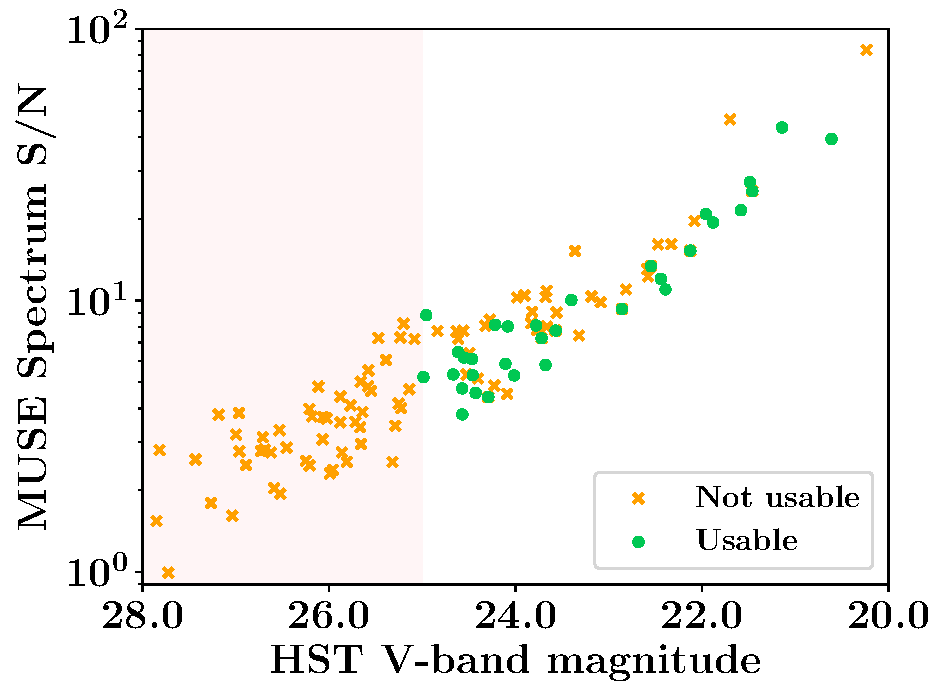
\includegraphics[width=0.5\textwidth]{data/sn_vs_vband}%
  }
  \caption[HUDF Objects]{\textit{Left-hand panel}: MUSE flux signal-to-noise (S/N) versus HST V-band magnitude for 252 extracted cubes. \textit{Right-hand panel}: Spectrum S/N versus HST V-band magnitude for reduced sample of extracted objects. \textit{Both}: final sample of 35 galaxies indicated as ``Usable'' (green), and the red area indicates the imposed magnitude limit of 25.0 mag, galaxies below this boundary had no visible [OII] emission feature present. The ``Not usable'' (orange) classification is a combination of either no [OII] feature and/or no visible absorption features.}
\label{fig:sn_vband}
\end{figure*}

Figure \ref{fig:sn_vband} demonstrates the sample reduction methods graphically where both plot the S/N versus V-band magnitude. However, the initial left-hand graph calculates the S/N from the flux and flux error provided by the MUSE catalogue, and the right-hand plot utilises the S/N calculated with the median and standard deviation of the region $(1+z)\times3700$ {\AA} to $(1+z)\times4500$ {\AA} in each galaxy spectra. This wavelength range was chosen as it was expected to contain the [OII] doublet and would be demonstrative of the signal. 

With a sample of high--redshift galaxies obtained, it was now possible to begin isolating and modelling the spectra emission and absorption features to test whether locally--derived scaling relations are valid. 

Note that within this paper, galaxies will be classified by their ID as defined by \texttt{SExtractor} (e.g., CXXXX), the corresponding Rafelski UVUDF ID is provided in Tables \ref{table:final_sample}, \ref{table:rest_of_final_sample}.

\vspace{2ex} % head space
\section{Discussion} \label{sec:discussion}
\subsection{Galaxy velocity dispersions} \label{sec:disc_vel_disp}
\noindent
To measure the gas and stellar kinematics of a galaxy, velocity dispersions were derived from modelling spectral features. 

Before both of these analyses were performed, a single spectra representing each galaxy was required. This was found by masking the galaxy data with the segmentation map, collapsing all voxels into a galaxy-integrated spectra, and then logarithmically binning the data using a routine found in the package \texttt{pPXF} \citep{2017MNRAS.466..798C}.

\vspace{2ex} % head space
\subsubsection{[OII] modelling} \label{sec:disc_oii_modelling}
\noindent
For the gas dynamics within these galaxies, the [OII] doublet was used as it is one of the brightest observable emission peaks at redshifts $0.3\lesssim z\lesssim 1.6$. To define the final sample of galaxies, a routine was ran to find whether the doublet could be found within the region $(1+z)\times3600$ {\AA} to $(1+z)\times3750$ {\AA}, and if the following Gaussian model could be fitted to the doublet,
\begin{multline}
f_{\text{[OII]}}(x) = cx + \frac{I_1}{\sigma \sqrt{2\pi}} \exp{\Bigg(-\frac{(x-L_1)^2}{2\sigma^2}\Bigg)} \\
+ \frac{I_2}{\sigma \sqrt{2\pi}} \exp{\Bigg(-\frac{(x-L_2)^2}{2\sigma^2}\Bigg)},
\label{eqn:doublet}
\end{multline} 

where $x$ are the redshifted wavelengths, ${c}$ is a constant, ${I_1}$ and ${I_2}$ are scaling factors limited by $I_1/I_2$, $L_1$ and $L_2$ are the [OII] peaks (3727.092, 3729.875 {\AA}) multiplied by $(1+{z})$ with $z$ as a free parameter, and $\sigma$ is the quadrature sum of a constant instrumental resolution $\sigma_{\text{inst}}$ and the deconvolved width of the doublet $\sigma_{OII}$ ($\sigma=\sqrt{{\sigma_{OII}}^2 + \sigma_{\text{inst}}^2}$).

For each fitting performed, the instrumental resolution was fixed to $\sigma_{\text{inst}}=45.4$ km s$^{-1}$. This width was calculated by fitting a Gaussian curve to the sky line found at 6000 {\AA} within a MUSE sky noise spectra. Additionally, the MUSE catalogue redshift would be used as an initial estimate for $z$.

\begin{figure}
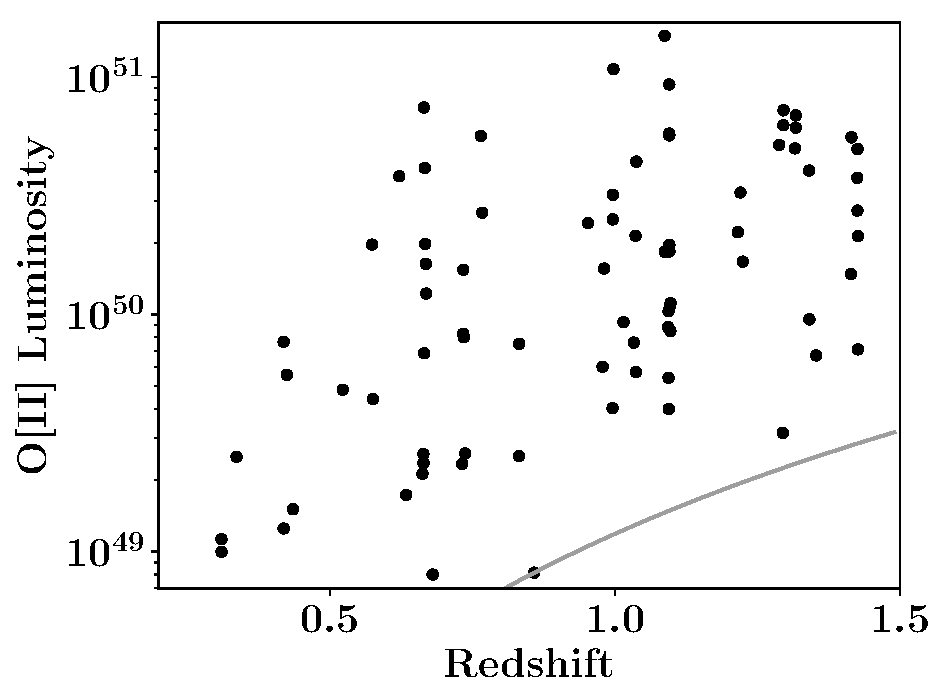
\includegraphics[width=1.0\linewidth]{data/o_ii_luminosity_vs_redshift}
\caption{[OII] luminosity against redshift for sample of 35 galaxies. Lower-limit of this sample (grey model) was calculated using the object with the smallest flux. All galaxies appear above this limit and approximately follow the luminosity-redshift trend. Note that objects with $z<0.3$ were not analysed as high--redshift galaxies were desired.}
\label{fig:oiiluminosity_redshift}
\end{figure} 

Organised by V-band magnitude, it was found that only 35 galaxies contained a visible [OII] emission doublet. This corresponded to a sample limiter of $\sim25.0$ mag. Subsequently, $f_{\text{[OII]}}$ calculated for these galaxies would be equivalent to the flux and [OII] luminosity of the peak. Plotting these luminosities against galaxy redshifts, as seen in Figure \ref{fig:oiiluminosity_redshift}, allows for the luminosity-redshift relation to be verified for the sample. This was desired as the returned parameters from the model fitting would be used to express galaxy kinematics and it was important to understand whether they reflected physical results. 

Tables \ref{table:final_sample}, \ref{table:rest_of_final_sample} provide the obtained gas velocity dispersions $\sigma_{OII}$ and redshifts $z$ for the galaxies. Quoted with each $\sigma_{OII}$ value is the fractional error. The returned errors from the Python model fitting package \texttt{lmfit} \citep{newville_matthew_2014_11813} were not used as their origins were dubious. The methodology used to produce the fractional errors is the following: the original best fitting velocity dispersions $\sigma_{best}$ and S/N between the CaH and H$\delta$ (4000 {\AA} to 4080 {\AA}) spectral lines were noted for the 10 brightest galaxies. The spectra for these galaxies were then perturbed 300 times with random normal noise based on the standard deviation between CaH and H$\delta$. The new spectra would be passed to the modelling fitting routine and the [OII] doublet would be fitted for. At each perturbation step, the new velocity dispersion $\sigma_{new}$ and corresponding S/N would be recorded. Then for every S/N value, the fractional error $\alpha_{\sigma_{OII}}$ could be calculated with, 
\begin{equation}
    \alpha_{\sigma_{OII}}=\frac{\mid \Delta \sigma \mid}{\sigma_{best}}=\frac{\mid \sigma_{best}-\sigma_{new} \mid}{\sigma_{best}}.
    \label{eqn:frac_error}
\end{equation}

\begin{figure*}
\centering
\subfloat{\label{fig:lmfit_sigma_frac_error_vs_sn}%
  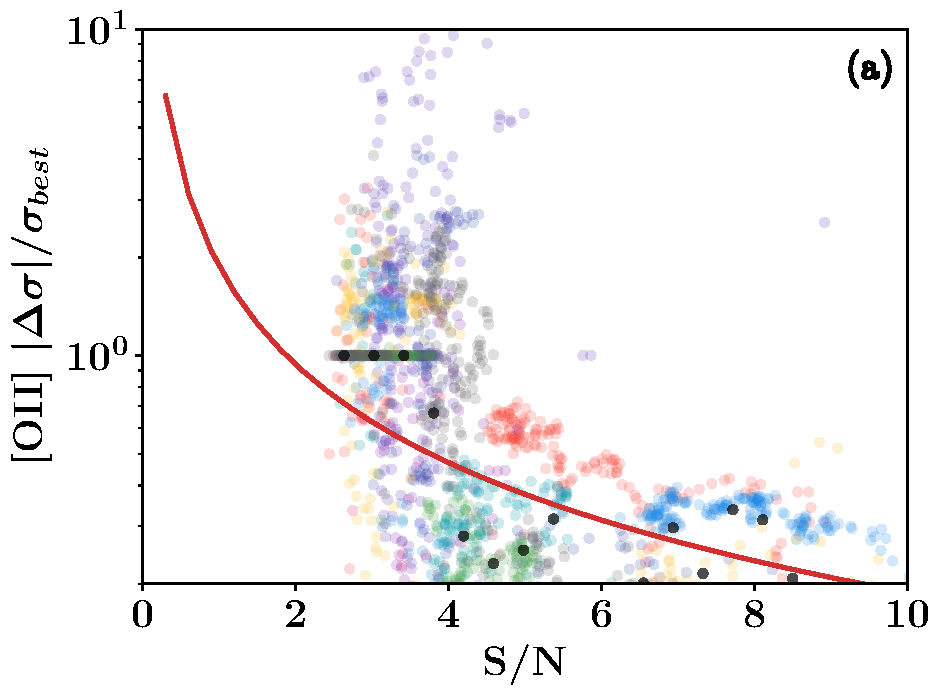
\includegraphics[width=0.495\textwidth]{data/lmfit_sigma_frac_error_vs_sn}%
  \label{fig:frac_err_oii_sigma}
  }
\subfloat{\label{fig:ppxf_sigma_frac_error_vs_sn}%
  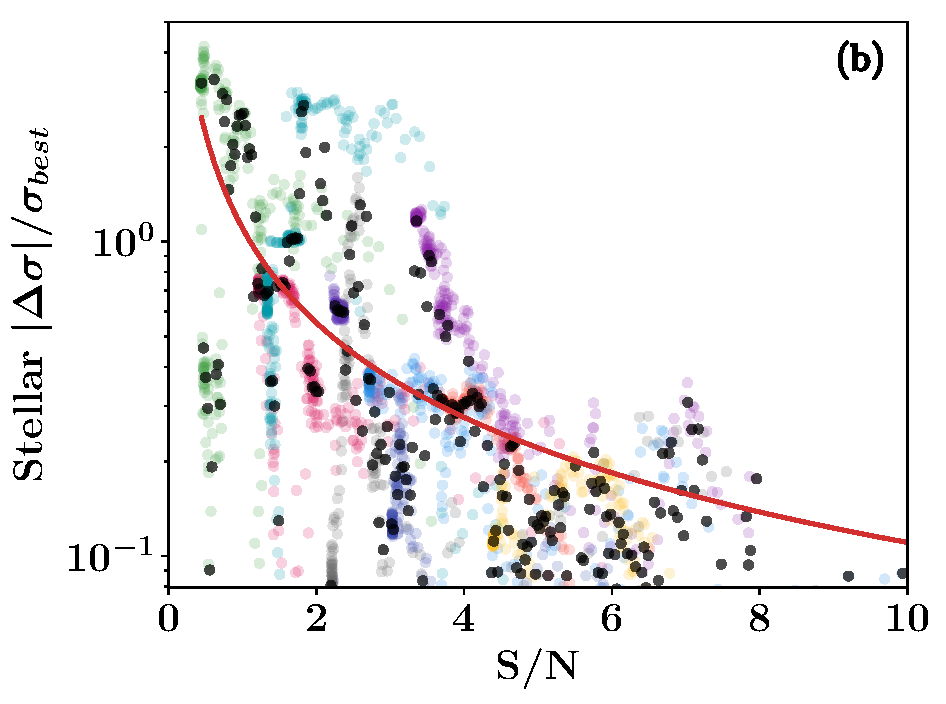
\includegraphics[width=0.495\textwidth]{data/ppxf_sigma_frac_error_vs_sn}%
  \label{fig:frac_err_stellar_sigma}
  }\\
\subfloat{\label{fig:lmfit_vel_frac_error_vs_sn}%
  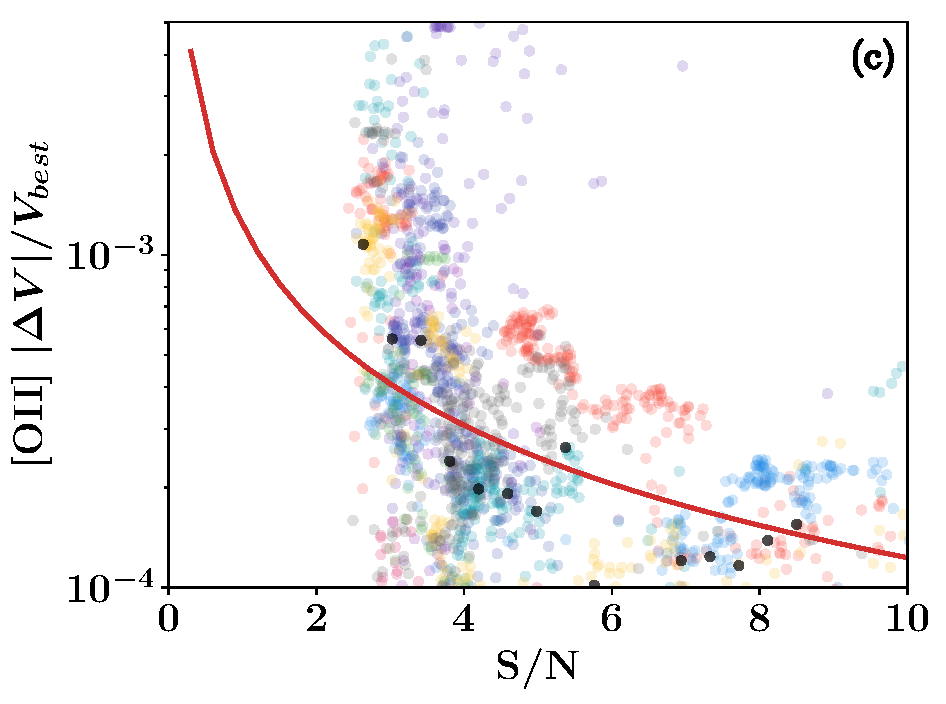
\includegraphics[width=0.495\textwidth]{data/lmfit_vel_frac_error_vs_sn}%
  \label{fig:frac_err_oii_vel}
  }
\subfloat{\label{fig:ppxf_vel_frac_error_vs_sn}%
  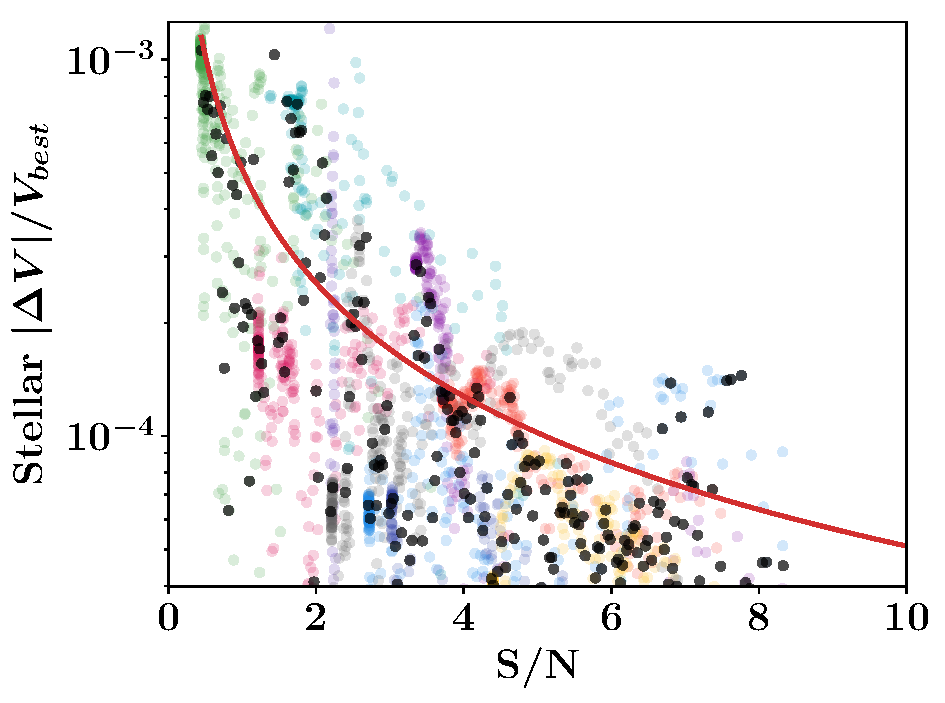
\includegraphics[width=0.495\textwidth]{data/ppxf_vel_frac_error_vs_sn}%
  \label{fig:frac_err_stellar_vel}
  }
\captionsetup{justification=raggedright}
\caption[Fractional uncertainties]{Fractional error models as a function of S/N for the gas and stellar velocity dispersions $\sigma$ and radial velocities $V$ obtained from \texttt{lmfit} and \texttt{pPXF} fitting routines. \ref{fig:fractional_errors}a--d: $a/x$ models (red) were derived to provide alternative uncertainties as the reliability and methodology of \texttt{lmfit} and \texttt{pPXF} was unknown and doubted. Obtained model parameters: (a) $a=1.88$; (b) $a=1.10$; (c) $a=0.00123$; and (d) $a=0.000510$.}
\label{fig:fractional_errors}
\end{figure*}

To create a quantified uncertainty value, the fractional error would be plotted against the S/N, and an $a/x$ model applied with $a$ as a scaling factor and $x$ as the S/N. Figure \ref{fig:frac_err_oii_sigma} provides the plot of the fractional error model for $\sigma_{OII}$ with $a=1.88$. 

Throughout this research, the fractional error method would be employed due to the undetermined nature of how model fitters produce uncertainties. It must be noted that the $z$ error values in the data tables are in fact the values from \texttt{lmfit}. It was decided that the fractional uncertainty method would not be directly applied for $z$, instead, later calculations of galaxy radial velocities which used $z$ would estimate overall fractional errors.

In an attempt to retrieve a secondary [OII] doublet width for comparison, an alternative fitter from \texttt{pPXF} was used. The spectra would be passed to the Python package and a gas fitting performed where major emission lines (e.g., [OII]3727,3729; [OIII]5007; etc.) would be detected and velocity plus velocity dispersions for each line returned. However, this test proved to be unsuccessful as the routine quickly deteriorated to produce $\sigma\approx1.0$ for a large majority of the cubes. It was suspected that this failed due to a lack of S/N for some cubes, and a failure in masking and fitting the [OII] line.

Instead, the \texttt{pPXF} fitting routine was used to measure the absorption features of the galaxy spectra. 

\vspace{2ex} % head space
\subsubsection{Absorption line modelling}
\noindent
With the gas kinematics of the high--redshift galaxies quantified by the [OII] emission line, a similar procedure of spectra modelling was applied to obtain the stellar kinematics from the absorption features.

The key tool within this analysis was the \texttt{pPXF} package. pPXF stands for penalised pixel-fitting and is used to perform parametric recovery of the line-of-sight velocity distribution of stars in a galaxy, whilst working in pixel space. The methodology was originally described by \cite{2004PASP..116..138C} and subsequently refined and upgraded in \cite{2017MNRAS.466..798C}. In essence, the \texttt{pPXF} routine utilises a stellar spectra template library to produce spectra models. Using spectra similar to those found in Figure \ref{fig:spectral_types}, varying numbers of templates are added together and manipulated in a $\chi^2$ reduction routine. Velocity and velocity dispersions for the stars can then be returned from these best fitting models.

The implementation of \texttt{pPXF} was in-part a black box routine, the data and parameters which could be passed to the procedure were: the logarithmically binned spectra, the $z$ for the galaxy, a noise spectra, a MUSE sky noise spectra, and a spectral template set. 

The noise spectra was generated by taking a region ($40\times 34$ pixel$^2$) in the segmentation map which appeared to be free of objects, then the standard deviation of each individual spectra pixel was calculated and then saved together as a noise spectra. 

In selecting a spectral template set, it had to be ensured that one with higher spectral resolution than MUSE ($\sim2.25$ {\AA} (FWHM)) was chosen. The Indo-US Library of Coud{\'e} Feed Stellar Spectra \citep{2004ApJS..152..251V} library with spectral resolution 1.35 {\AA} (FWHM) was selected due to the wide wavelength coverage (3460--9464 {\AA}) and the large spectral resolution. 

\begin{figure*}
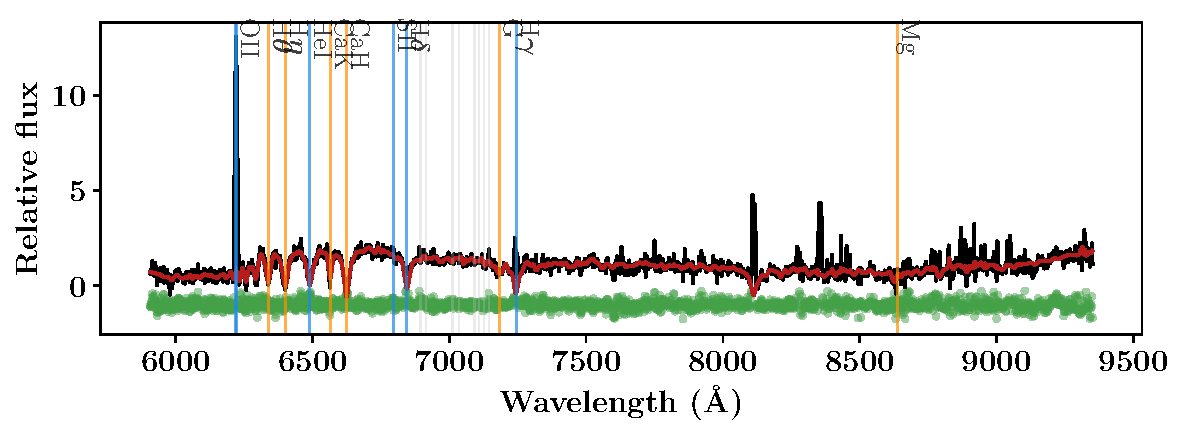
\includegraphics[width=\textwidth]{data/cube_1804_spectra_complete}
\caption{Spectra and best fitting \texttt{pPXF} model for C1804. The galaxy integrated spectra (black) was passed to the \texttt{pPXF} fitting routine which would normalise the data and return a best fitting model (red) plus values for galaxy radial velocity and velocity dispersion. The residuals between the data and model (green) are shown in addition to highlighted emission (blue), absorption (orange), and iron (grey) spectra features. For C1804 in particular, \texttt{pPXF} provided a reduced $\chi^2 \approx 1.69$ which indicates a good fit.}
\label{fig:ppxf_spectra}
\end{figure*}

After the fitting routine was set up and ran, \texttt{pPXF} was able to return radial velocity and velocity dispersion values for the galaxy stellar component, and output the best-fitting model. Figure \ref{fig:ppxf_spectra} provides an example of the optimum fitting with galaxy C1804. It appeared that \texttt{pPXF} was able to provide a good fitting to the spectral data as the calculated $\chi^2_\nu\approx1.69$. However it was indicative to perform various tests and other forms of analysis to verify the reliability of the returned parameters. 
 
As with \texttt{lmfit}, \texttt{pPXF} would return values with accompanied uncertainties, and again, their origins were questioned so a fractional error model was created for the stellar velocity dispersions. Figure \ref{fig:frac_err_stellar_sigma} was produced with same methodology as described in Section \ref{sec:disc_oii_modelling}, but stellar velocity dispersions were now used $\sigma_*$ and a new fitted model with $a=1.10$. 

The stellar velocity dispersions and their associated uncertainties can be found in Table \ref{table:final_sample}. It can be immediately seen that it was not possible to run \texttt{pPXF} for the entire final sample of 35 galaxies. With C109 through C1225 found in Table \ref{table:rest_of_final_sample} in Appendix \ref{appendix:rest_of_final_sample}, these galaxies (20 objects) were found to not have enough S/N in their absorption features (hence their separation from the main report). This resulted in a smaller potential sample for the comparison of the stellar and gas kinematics in galaxies. 

If the $\sigma_*$ values are examined for the remaining 15 galaxies, certain results are questionable. C849, C549, and C895 are three objects in particular which stand out because of their unlikely low values of $\sigma_*\lesssim 25$ km s$^{-1}$. Comparing this with the calculated value for the MUSE instrumental resolution $\sigma_{\text{inst}}=45.4$ km s$^{-1}$, it is dubious that \texttt{pPXF} was able to reconstruct information which would have been lost due to instrumental convolution. 

This therefore required the introduction of further sample reduction techniques to ensure that only reliable results were obtained. Employing the MUSE instrumental resolution $\sigma_{\text{inst}}/2$ (the FWHM/2), $\sigma_{\text{pPXF--limit}} \approx22.7$ km s$^{-1}$ was introduced as a lower limit in which \texttt{pPXF} would not be able to reconstruct velocity dispersions. Additionally, it was decided that the sample should be further restricted by the S/N of the galaxy. This was defined with the fractional error model for the stellar velocity dispersions, galaxies with S/N $\lesssim 4$ would correspond to a fractional error of $\gtrsim 27.5\%$. Beyond this percentage, the uncertainties were deemed too large and the connected result would become meaningless. 

\begin{table}
\begin{center}
\begin{tabular}{c@{\hskip 20pt}c@{\hskip 20pt}c} 
\hline
\textbf{Cube ID} & \textbf{S/N} & \textbf{$\boldsymbol{\sigma_*}$ (km s$^{-1}$)} \\ [0.5ex] 
C1804 & 7.95 & $182(25)$ \\

C1578 & 10.4 & $117(12)$ \\

*C849 & 6.06 & \emph{3.8(7)} \\

C286 & 10.5 & $58(6)$ \\

C5 & 8.80 & $78(10)$ \\

C767 & 7.85 & $148(21)$ \\

C414 & 5.68 & $106(21)$ \\

*C549 & 4.95 & \emph{25(6)} \\

C175 & 5.60 & $127(25)$ \\

C1129 & 4.38 & $60(15)$ \\

C765 & 6.02 & $65(12)$ \\

*C1075 & \emph{3.86} & $143(41)$ \\

C540 & 6.96 & $60(10)$ \\

*C895 & \emph{3.59} & \emph{0.5(2)} \\

C554 & 6.85 & $123(20)$ \\
 \hline
\end{tabular}
\caption{Galaxy cube ID, S/N, and stellar velocity dispersion values returned from \texttt{pPXF} for 15 galaxies. These were galaxies which could be parsed and analysed by \texttt{pPXF}, however, not all the results are valid. Galaxies which are marked by * indicate that galaxy was disregarded with the reason demonstrated by the underlined S/N and/or $\sigma_*$ values.}
\label{table:ppxf_sigma_sn}
\end{center}
\end{table}

Table \ref{table:ppxf_sigma_sn} provides the 15 galaxies which could be analysed by \texttt{pPXF}. Marked in this table are four particular galaxies which were considered unusable due to the enforced S/N and $\sigma$ cut-offs. It can be seen that the uncertainties for these galaxies were severely underestimated due to the corresponding low $\sigma_*$ value. In these scenarios it appeared that the \texttt{pPXF} uncertainties were better estimates than the fractional error (e.g., C849: $\sigma_{\text{pPXF}}=3.8(58)$ cf. $\sigma_{\text{FE}}=3.8(7)$), however their origins are still doubtful.

As a comparison and test of the \texttt{pPXF} $\sigma_*$ results, attempts were made to model the CaH and CaK absorption lines. Located at $3934.777\times(1+z)$ {\AA} and $3969.588\times(1+z)$ {\AA}, both of these lines are Voigt profiles and not Gaussian like the [OII] doublet. A model was created in \texttt{lmfit} using inbuilt model profiles,
\begin{multline}
    \texttt{Linear($c$) + Voigt($A_1$, $\mu_1$, $\sigma$)} \\ 
    \texttt{+ Voigt($A_2$, $\mu_2$, $\sigma$)},
    \label{eqn:voigt_model}
\end{multline} 

where $c$ is a constant, $A_1$ and $A_2$ are the Voigt amplitudes, $\mu_1$ and $\mu_2$ are the locations of the peaks, and $\sigma$ is the quadrature sum of the instrumental resolution $\sigma_{\text{inst}}$ and width of the Voigt profiles $\sigma_{\text{Voigt}}$ ($\sigma=\sqrt{\sigma_{\text{inst}}^2 + \sigma_{\text{Voigt}}^2}$). 

\begin{figure*}
  \subfloat{\label{fig:voigt_cah_cak}%
  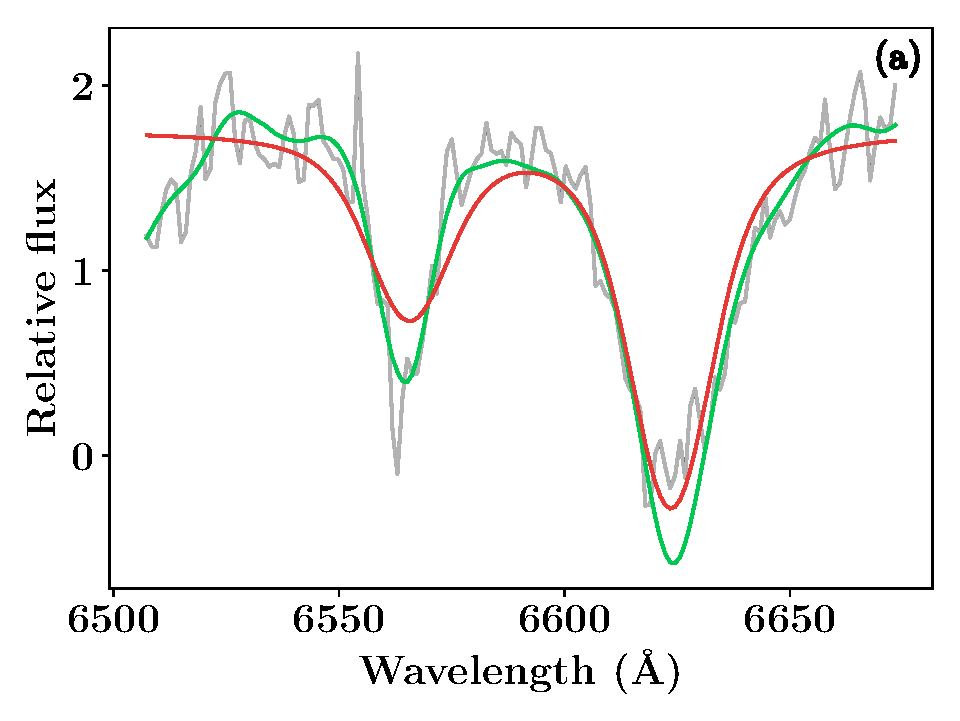
\includegraphics[width=0.5\textwidth]{data/voigt_cah_cak.pdf}
  }
  %
  \subfloat{\label{fig:voigt_cak}%
  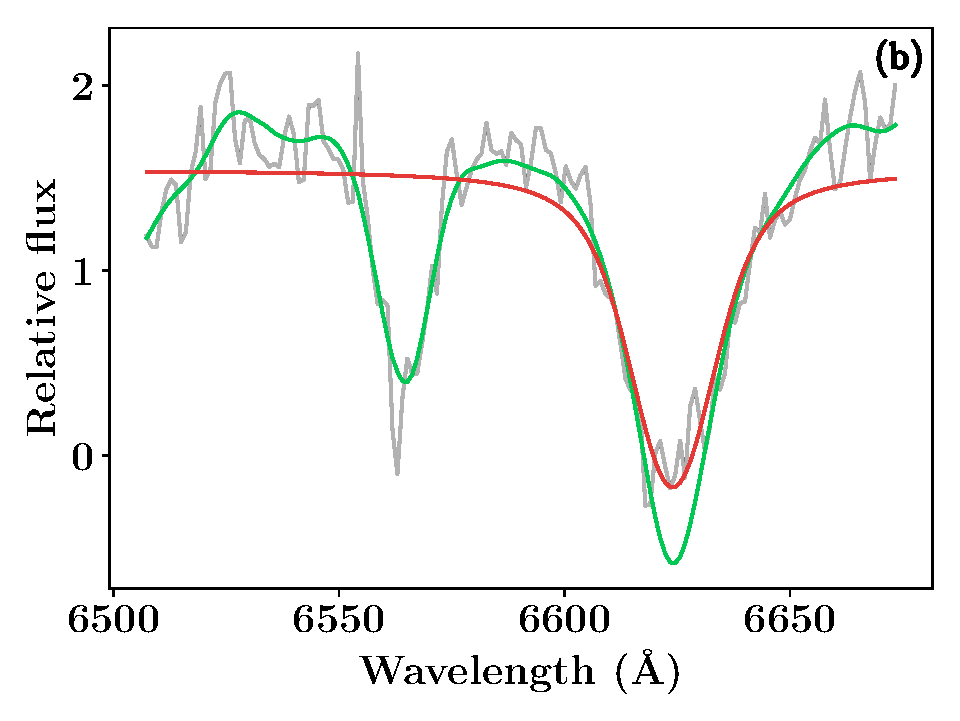
\includegraphics[width=0.5\textwidth]{data/voigt_cak.pdf}
  }
  \caption[Voigt modelling]{Attempts at Voigt modelling for CaH and CaK spectral absorption lines for C1804. The working region $3900\times(1+z)$ {\AA} to $4000\times(1+z)$ {\AA} was isolated from the data (grey), overlaid is the best fitting \texttt{pPXF} model (green), and (a) and (b) utilise two different models (red). (a) uses the model found in Equation \ref{eqn:voigt_model} with two Voigt profiles. (b) employs a reduced model of just one Voigt profile in an attempt to simplify the testing.}
\end{figure*}

It was found that with a standard fitting: i.e., selecting out C1804, isolating the spectral region $3900\times(1+z)$ {\AA} to $4000\times(1+z)$ {\AA}, and running \texttt{lmfit} with the Voigt model; the produced fit (Figure \ref{fig:voigt_cah_cak}) appeared to match the general locations of the spectral lines, and the overall profile for CaK. 

The produced velocity dispersion for this fit was $\sigma_{\text{Voigt}}=281(18)$ km s$^{-1}$, where the uncertainties were obtained from \texttt{lmfit}. The quality of fit ($\chi^2_\nu=0.0704$) did not warrant a fractional uncertainty model to be produced. Comparing $\sigma_\text{Voigt}$ with $\sigma_*$ for C1804, both values are clearly not within range of each other which prompted for a simpler model of just one Voigt profile and a linear component to test whether that could return similar values.

Excluding CaH, Figure \ref{fig:voigt_cak} is the fitting with the reduced model. Whilst it looked like the general profile for CaK was still fitted for, the returned velocity dispersion $\sigma_{\text{Voigt}}=289(31)$ km s$^{-1}$ was now further away from the \texttt{pPXF} result. Whilst further improvements could be made to the fitting: i.e., removing the baseline of the data, applying additional constraints, and producing custom Voigt models; it was deemed a wasteful use of time to pursue a replication of \texttt{pPXXF} which had taken several year's worth of research to create. Therefore, the values from \texttt{pPXF} were accepted from the results of testing the uncertainties, and the work in finding the optimal stellar template library. 

\vspace{2ex} % head space
\subsubsection{$\sigma$ comparisons}
\noindent
The sample of 11 analysed high--redshift galaxies and their obtained velocity dispersions were naturally used to compare the stellar and gas kinematics. 

\begin{figure}
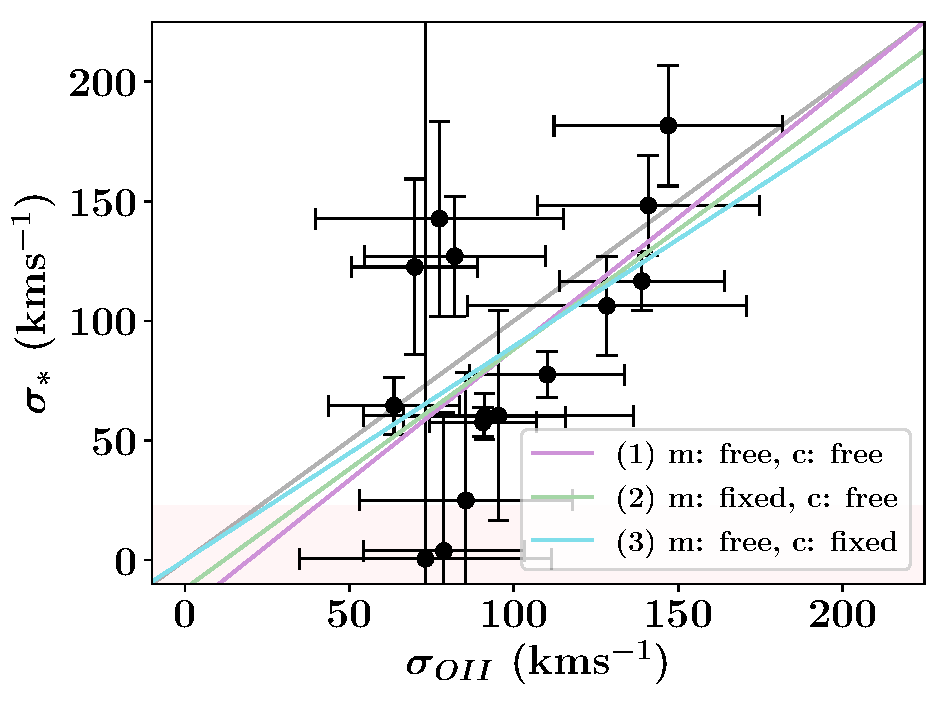
\includegraphics[width=1.0\linewidth]{data/sigma_star_vs_sigma_oii}
\caption{Gas velocity dispersions $\sigma_{OII}$ against stellar velocity dispersions $\sigma_*$ for a sample of 11 galaxies (black). Included are four galaxies (red) C849, C549, C1075, and C895 marked with their original \texttt{pPXF} errors. These objects were removed from the sample due to low S/N or because of the $\sigma_*$ limit imposed by the instrumental limitation of MUSE (red region, FWHM/2$=\sigma_*=22.7$ km s$^{-1}$). Three linear models were fitted to the data: (1) free gradient and free intercept, $\chi^2_{\nu}=6.48$; (2) fixed gradient and free intercept, $\chi^2_\nu=6.03$; and (3) free gradient and fixed intercept, $\chi^2_\nu=5.87$. Linear model 3 appears to be the best fit with the lowest $\chi^2_\nu$ and it makes the most physical sense, i.e, if there are no gas dynamics then there should be no stellar dynamics.}
\label{fig:velocity_dispersions}
\end{figure}

Figure \ref{fig:velocity_dispersions} plots the sample of galaxies from Table \ref{table:ppxf_sigma_sn}. The four objects which were removed from the analysis are included to demonstrate how they compare with the other galaxies. 

The first form of analysis performed on the kinematic data was quantifying how well a linear model could be fitted. Three models were tested: free gradient and free intercept, fixed gradient and free intercept, and free gradient and fixed intercept. When fitted to the data, the latter model appeared to be the best fit as it produced the smallest reduced $\chi^2$ statistic of $\chi^2_\nu=5.87$. From the presented data and within their uncertainties, the galaxies do appear to follow the linear trend. Nonetheless, the offsets still must be questioned and it should be investigated whether there is a physical reason for the galaxies to deviate. 

The median ratio $\sigma_{OII}/\sigma_*$ has a value of 1.19 (with standard deviation $\sim0.35$) which could be used to indicate an offset in the scaling relations between the stars and gas, however with the calculated uncertainties this could instead imply that the scaling relations do in fact agree. 

The next logical line of inquiry would be to examine whether the offsets are being driven by galaxy morphology. For the sample of galaxies within Figure \ref{fig:velocity_dispersions} (including the eliminated four), they all appeared to be spiral types with features such as spiral arms, a defined disc plane, and a central nucleus bulge. So one could conclude that the general galaxy type is not prompting the materialisation of the offset. 

\begin{figure}
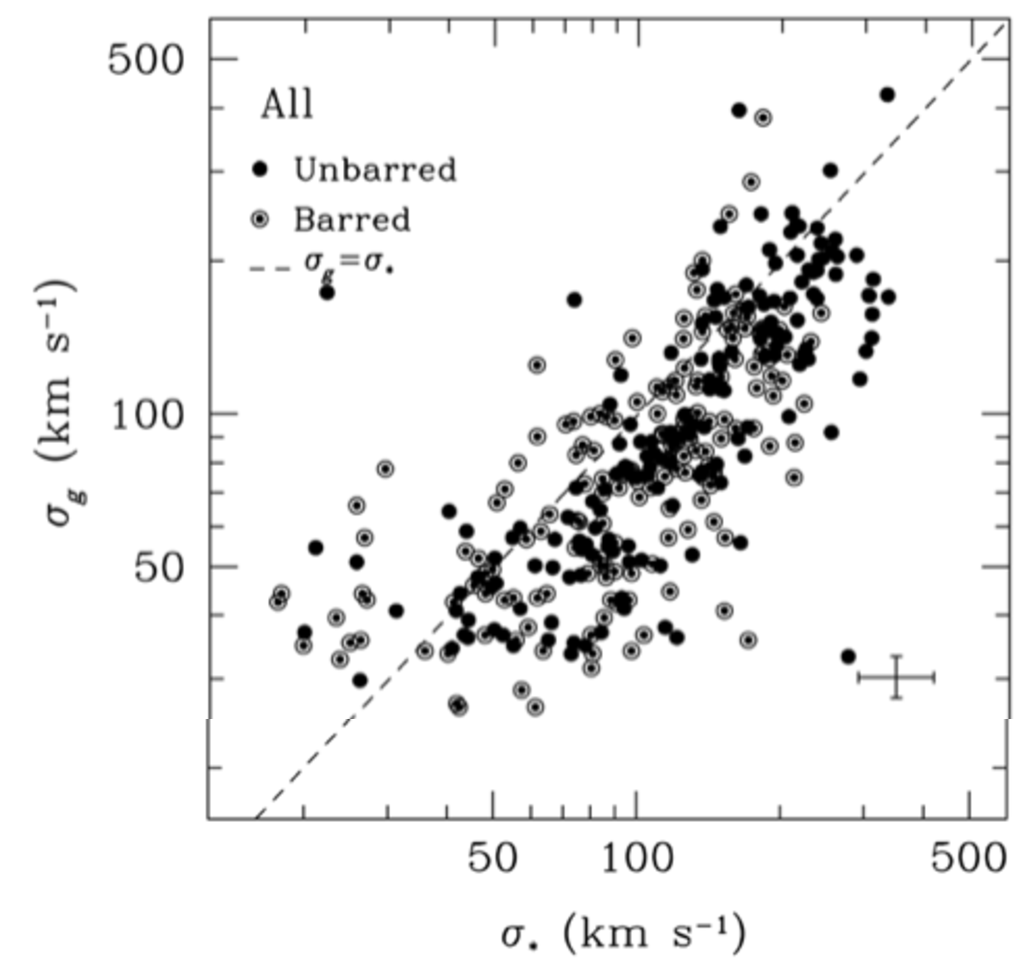
\includegraphics[width=1.0\linewidth]{data/ho_2009.pdf}
\caption{Gas $\sigma_g$ and stellar $\sigma_*$ velocity dispersion distribution for 345 galaxies of elliptical, lenticular, and spiral type from the Palomar spectroscopic survey (from \cite{2009ApJ...699..638H}). All galaxy types appear to demonstrate the same correlated kinematics. }
\label{fig:ho_2009}
\end{figure} 

Figure \ref{fig:ho_2009} provides a comparative plot of galaxy stellar and gas kinematics produced by \cite{2009ApJ...699..638H}, where a sample of 345 nearby galaxies ($z\lesssim0.5$) were taken from the Palomar spectroscopic survey \citep{1995ApJS...98..477H, 1997ApJS..112..315H}. One of the main differences in their work is that they quantified the gas kinematics through the [NII]$\lambda6583$ emission line due to the spectral range of the double spectrograph on the Hale telescope ($\sim$4230--5110 {\AA} and $\sim$6210--6860 {\AA}). Through splitting their galaxy sample into the various Hubble types (ellipticals, spirals, and lenticulars), they concluded that the correlation found between gas and stellar velocity dispersions for the entire sample is also replicated for the individual galaxy types. The previous suggestion of different morphological types driving variances in the kinematics is now looking more unlikely, however, at higher--redshifts the dynamics may potentially behave differently. 

Another disparity between the work of \cite{2009ApJ...699..638H} and the research presented here, is the model applied to their data. With a larger sample at hand they were able to recognise that a simple Gaussian was considered a suitable fit to their data. In this work, it is difficult to draw similar conclusions when the sample is limited to 11 galaxies. 

\begin{figure}
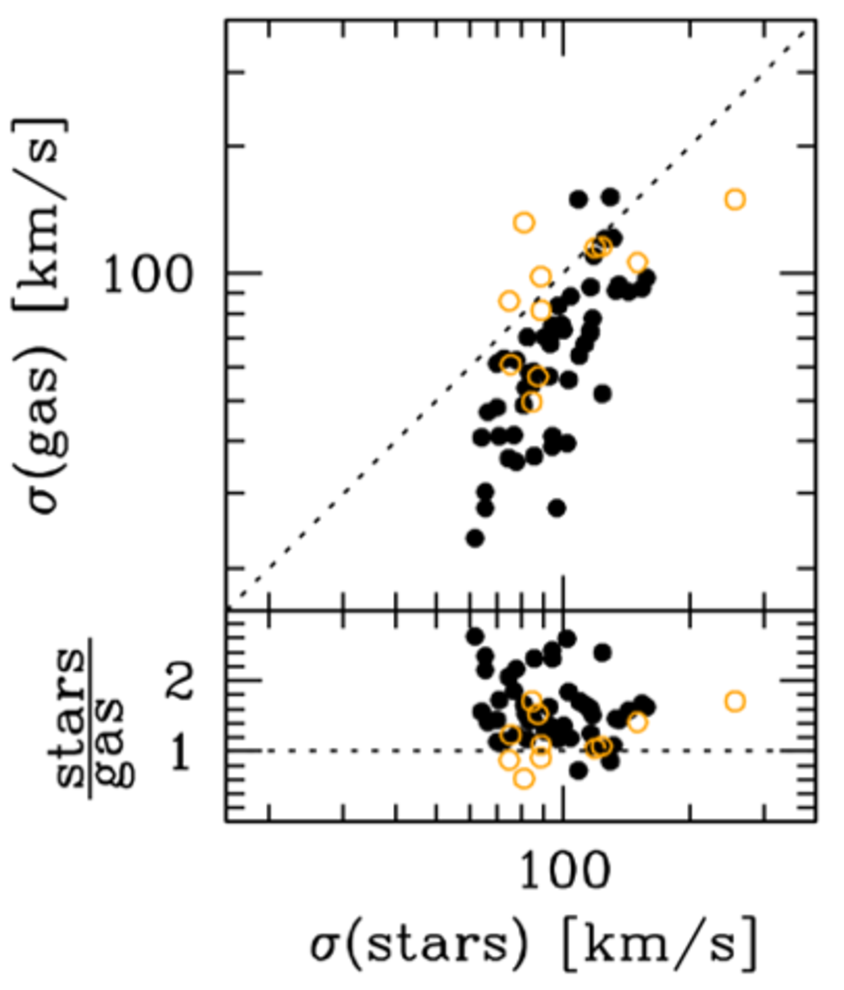
\includegraphics[width=0.6\linewidth]{data/cortese_2010.pdf}
\caption{Gas $\sigma$(gas) and stellar $\sigma$(stars) velocity dispersion distribution for 62 galaxies from the SAMI galaxy survey (from \cite{2014ApJ...795L..37C}). Data shows an offset of the gas velocity dispersions from the $\sigma$(gas)=$\sigma$(stars) line.}
\label{fig:cortese_2010}
\end{figure} 

Alternative comparisons can be made with the work of \cite{2014ApJ...795L..37C}. Shown in Figure \ref{fig:cortese_2010} are 62 low--redshift ($0.004<z<0.095$) objects from the SAMI galaxy survey, their work aimed to demonstrate the possibility of a unified dynamical scaling relation for all galaxy types. What is of particular interest is their result for the kinematics between gas and stars. They derived that whilst the stars and gas scaling relations appear to be correlated, they are also offset with $\sigma(gas)$ is lower than $\sigma(stars)$ by a factor of 0.19 dex. \cite{2014ApJ...795L..37C} were able to utilise 11 emission lines ([OII]$\lambda\lambda$3726,29; H$\beta$; [OIII]$\lambda\lambda$4959,5007; [OI]$\lambda$6300; [NII]$\lambda\lambda$6548,83; H$\alpha$; and [SII]$\lambda\lambda$6716,31) to derive their gas velocity dispersions, something which is difficult to achieve with high--redshift data. 

Comparing the results of both \cite{2009ApJ...699..638H} and \cite{2014ApJ...795L..37C} to the research presented in this paper, it is difficult to draw certain and conclusive statements due to the limited nature of the high--redshift galaxy sample. But it does appear that the [OII] gas and stars follow a correlation which provides an indication that the [OII] emission doublet is valid for investigating the applicability of scaling relations at high--redshifts.

\begin{figure}
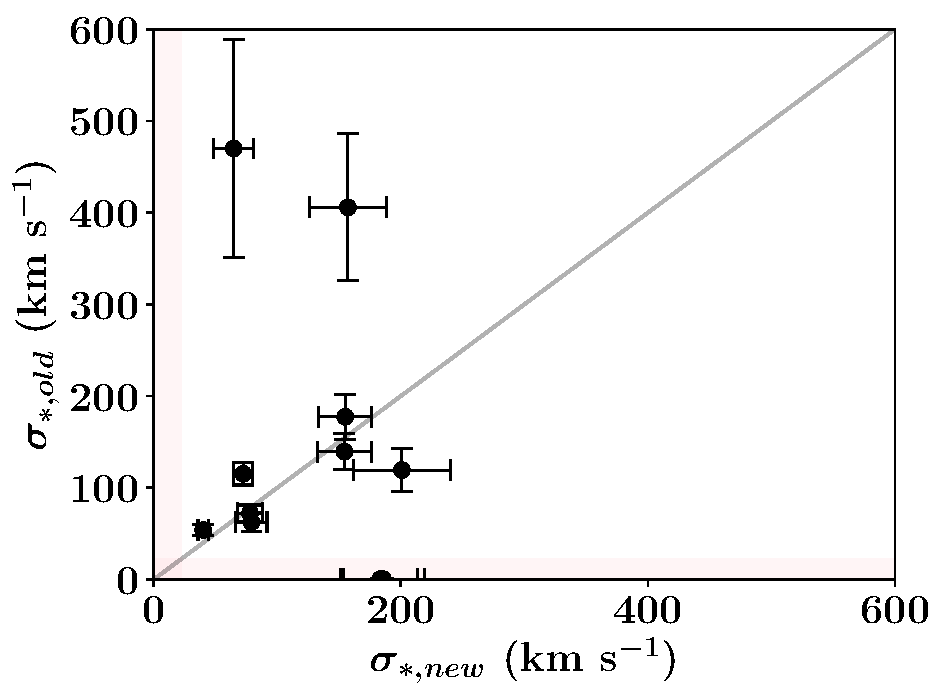
\includegraphics[width=1.0\linewidth]{data/sigma_stars_old_vs_new}
\caption{Velocity dispersions for old (\textit{GK}) versus young (\textit{OA}) stellar types. 11 galaxy spectra were isolated into overlapping regions of $3700\times (1+z)$ {\AA} to $4200\times(1+z)$ {\AA} for young stars, and $4000\times (1+z)$ {\AA} to $4500\times(1+z)$ {\AA} for old stars. If a linear trend is considered then C1129 and C175 strongly deviate from this line. This could be attributed to the difficulty in fitting for smaller wavelength regions or to problems with high noise. }
\label{fig:velocity_dispersions_old_new}
\end{figure} 

It was then subsequently tested whether the kinematics of different stellar populations within galaxies could be separated and demonstrated as a scaling relation. Figure \ref{fig:velocity_dispersions_old_new} shows the attempt made at separating old \textit{GK} and young \textit{OA} stellar types. The spectra was split into two regions ($3700\times (1+z)$ {\AA} to $4200\times(1+z)$ {\AA} and $4000\times (1+z)$ {\AA} to $4500\times(1+z)$ {\AA}) and then individually passed to the \texttt{pPXF} routine. What is striking are the points with $\sigma_{*,old}>300$ km s$^{-1}$ and $\sigma_{*,old}\approx0$. This demonstrates clearly \texttt{pPXF}'s inability to achieve reputable results when presented with spectra which do not contain enough information. If the dynamics of the gas and stars were seen to correlate (Figure \ref{fig:velocity_dispersions}), then it would be unsurprising to find that the dynamics of old and young stars correlate. Seven of the galaxies from the sample indicate this. 

\vspace{2ex} % head space
\subsection{Galaxy velocities}
\noindent
Revisiting the validity of the stellar and gas results from \texttt{lmfit} and \texttt{pPXF} for the final derived sample of 11 galaxies. The galaxy radial velocities can be derived and compared. 

\begin{figure}
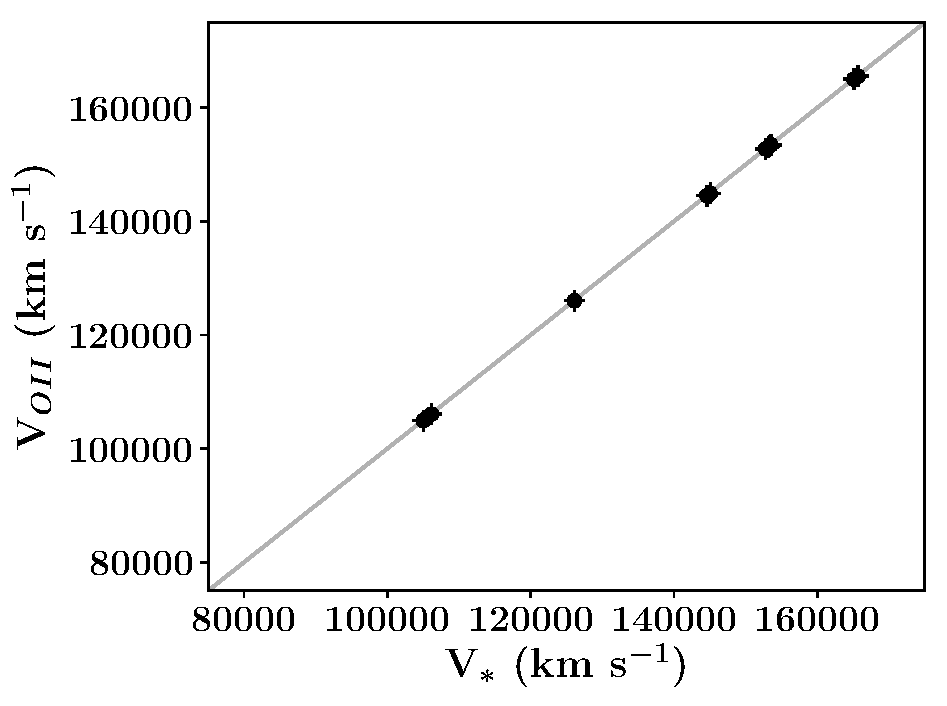
\includegraphics[width=1.0\linewidth]{data/vel_star_vs_vel_oii}
\caption{Stellar and [OII] gas velocities for 11 galaxies. The calculated velocities appear to be well in agreement with each other with only a $0.0757\%$ fractional difference. Both components appear to move with approximately the same radial velocity.}
\label{fig:velocities}
\end{figure}

Both routines make use of logarithmically binned spectra to derive values for galaxy redshifts, then the following equation is used to find radial velocities,
\begin{equation}
    V=c\ln(1+z),
\end{equation}

where $c$ is the speed of light, and $z$ is the obtained galaxy redshift. Figure \ref{fig:velocities} shows that by appearance, the calculated velocities appear to be well in agreement. This is the expected result as the stars within the galaxies should trace approximately the same radial velocities as the gas. 

For these velocities, fractional error models were additionally produced as seen in Figures \ref{fig:frac_err_oii_vel}, \ref{fig:frac_err_stellar_vel} with the stellar error model using $a=0.000510$ and [OII] with $a=0.00123$. These uncertainty models were naturally generated as the unsurety surrounding \texttt{lmfit} and \texttt{pPXF}'s generation of errors still permeated.

\vspace{2ex} % head space
\subsection{Voronoi tessellation}
\noindent
With the fitting routines validated by the velocity dispersion and velocity correlations, it was then proposed whether it was possible to subdivide the galaxy map to individually test the Tully--Fisher and Faber--Jackson scaling relations.

This process of binning the 2D galaxy map was performed with the package \texttt{VorBin}. As described in \cite{2003MNRAS.342..345C} and \cite{2009arXiv0912.1303C}, this routine would tessellate a galaxy map into bins based on the constraint of a minimum target S/N. Starting from the central pixel, the bins would ``bloom'' out and cover the entire galaxy. With the binned map, spectra could be produced for each smaller region and subsequently passed to \texttt{lmfit} and \texttt{pPXF} to produce various maps such as the radial velocity and velocity dispersions of galaxies.

To ensure that only the galaxy was binned, the segmentation maps were initially applied as a mask to the data. Then applying \texttt{VorBin} to the sample of 11 galaxies, it was found that only six objects could be tessellated. The routine would struggle to bin the 2D maps for the dimmer galaxies as they would not contain enough S/N. 

The Voronoi target S/N for each galaxy was chosen so that $\sim50$ bins would be produced for each galaxy. This value was selected as it was found to separate the galaxies into enough discernible individual regions. Later S/N masking would increase the difficulty in analysing the scaling relations at high--redshift.

\vspace{2ex} % head space
\subsubsection{Tully--Fisher} \label{sec:voronoi_tully_fisher}
\noindent
To test the Tully--Fisher relation, the end objective was to generate galaxy rotation curves and achieving this required galaxy velocity maps. 

The first step was to mask the Voronoi map and remove bins with S/N$<4$, this limit was imposed in the previous galaxy sample reduction and the reasoning is still valid here. Below this value there would not be enough information to reconstruct the galaxy kinematics. The reduced data array would then be passed to the [OII] and stellar routines and subsequent velocity maps produced from their results. The radial velocities for the central Voronoi bin was taken away from each map to produce rotational velocities. 

\begin{sidewaysfigure*}
\vspace{50ex}
%\centering
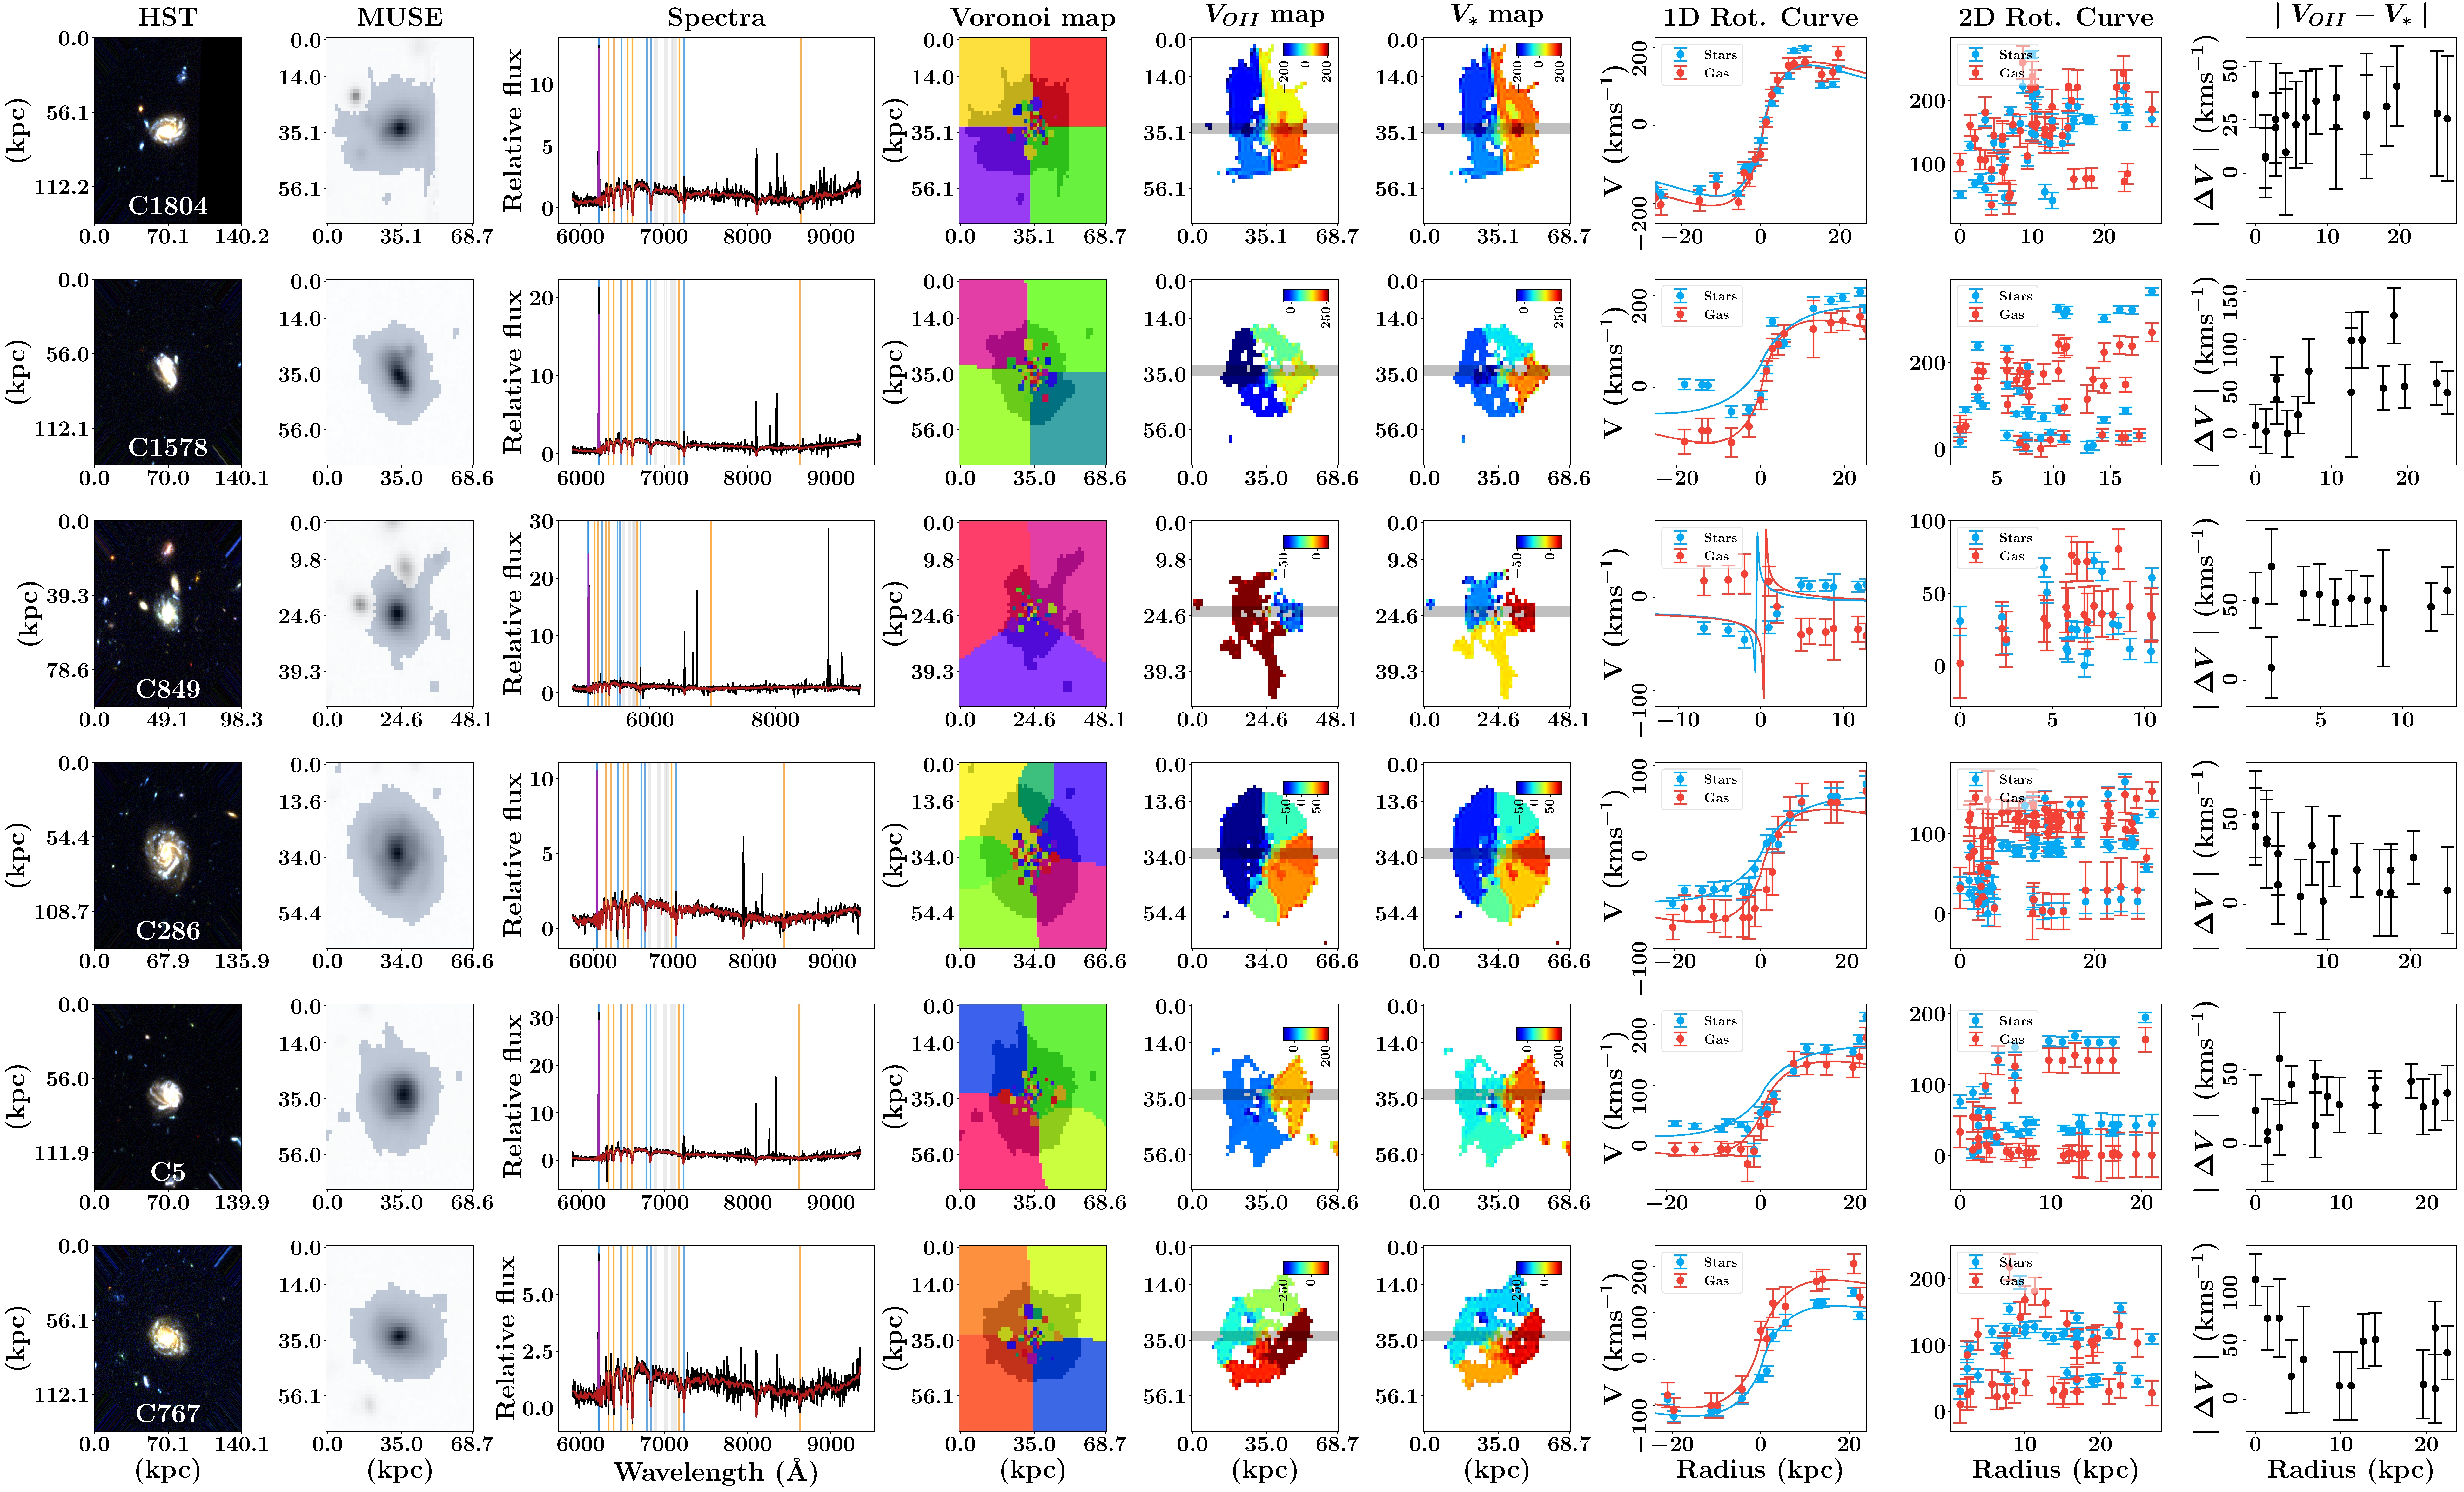
\includegraphics[width=1.0\textheight,height=0.6\textwidth]{data/spectra_complete_velocities}
\caption[Tully-Fisher]{Voronoi tessellation analysis for six galaxies. \textit{HST}: HST image and galaxy ID. \textit{MUSE}: 2D MUSE optical image and segmentation area (grey). \textit{Spectra}: galaxy data (black); \texttt{pPXF} model (red); and emission (blue), absorption (orange), and iron (grey) spectral lines. \textit{Voronoi map}: Voronoi tessellated map of galaxy, segmentation area, and the target S/N with achieved bin number in brackets. \textit{$V_{OII}$, $V_{*}$ maps}: velocity fields for galaxy. \textit{1D Rot. Curve}: rotation curve as defined by grey slice on the velocity maps. \textit{2D Rot. Curve}: rotation curves derived from every galaxy inclination-corrected maps. \textit{$\mid V_{OII}-V_* \mid$}: absolute difference of gas and stellar velocities versus galaxy radius using data from 1D rotation curves.}
\label{fig:multiple_spectra_tully_fisher}
\end{sidewaysfigure*}

Before the curves could be produced, the major kinematic axis of the galaxies were rotated and aligned across the horizontal. The major kinematic axis would not necessarily align with the major morphological axis so discretion was used to rotate the maps. This procedure was applied using a combination of the returned angle from horizontal from the previous \texttt{SExtractor} results, and in-part by manually adjusting until the axis was aligned horizontally. 

Once rotated, two rotation curves were produced. The first was ``1D'' where a 40 pixel height slice was taken across the width of the galaxy major kinematic axis and the velocities stored for each bin in that slice. The second curve was ``2D'' and sought to utilise the velocities from every bin for the galaxy. This was desired in a hope to improve the profiles seen from the 1D curves. However, as not all galaxies are observed face-on, their velocities and radii had to be corrected for inclination. Using the following to correct for velocities,
\begin{equation}
V_{los} = V_{rot} \cos{i},    
\end{equation}

where $V_{los}$ is the line of sight velocity, $V_{rot}$ is the corrected velocity, and $i$ is the inclination found using the semi-major ($b$) and semi-minor ($a$) parameters from the \texttt{SExtractor} routine ($\cos{i}=b/a$). 

The radii to each bin was corrected using,
\begin{equation}
    R_{corr}^2 = R_{obs}^2 + R^2_{y,obs} \tan^2{i},
\end{equation}

with $R_{corr}$ as the corrected radius, $R_{obs}$ is the measured radius, $R_{y,obs}$ is the $y$ component of the measured radius, and $i$ is the inclination angle \citep{2017_helen}. Note that this equation is only valid if the maps have been rotated so that the major kinematic axis is aligned horizontally.

Figure \ref{fig:multiple_spectra_tully_fisher} demonstrates the produced segmentation map, velocity maps, the 1D and 2D rotation curves, and the absolute differences between the 1D gas and stellar velocities. Galaxy C849 appears to have it's velocity dynamics flipped, however this could either be a result of low binning or a demonstration of counterrotating gas and stars. Nevertheless, it appears that 1D rotation curves could be produced for the six galaxies, with the 2D method struggling as noise from non-galaxy bins failed to be masked. 

\begin{figure}
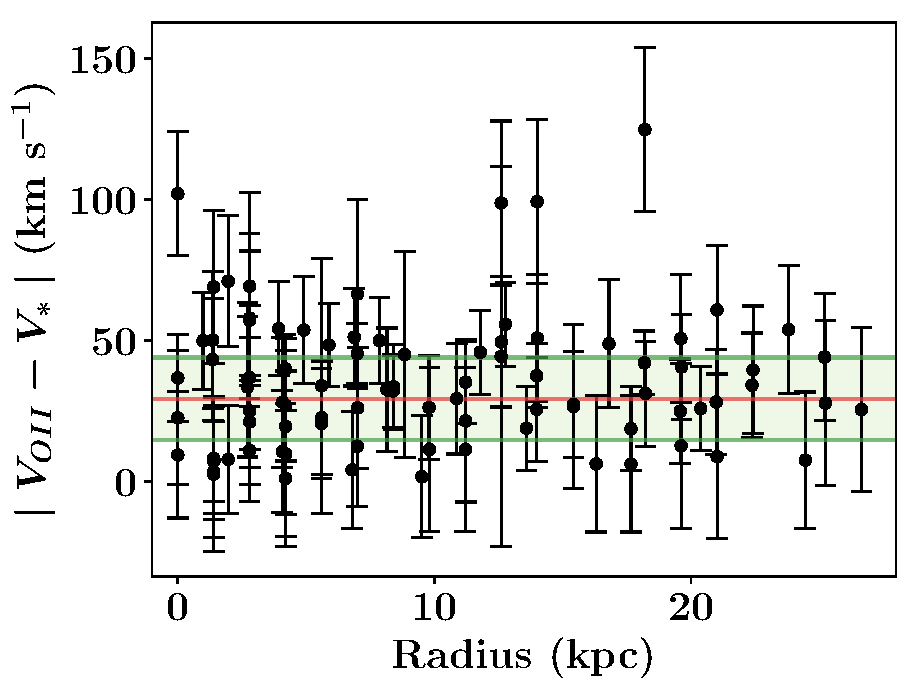
\includegraphics[width=1.0\linewidth]{data/deltav_vs_radius.pdf}
\caption{The absolute differences between the rotation velocities for the [OII] gas and stars for six galaxies as a function of galaxy radius. The median 29.5 km s$^{-1}$ is marked (red) along with the area equalling $1\sigma$ (green). There appears to be a systematic offset between both galaxy components.}
\label{fig:rotation_velocity_differences}
\end{figure} 

The absolute offsets between the [OII] gas and stellar rotation velocities were collated for the six galaxies to produce Figure \ref{fig:rotation_velocity_differences}. This plot suggests that there is a systematic offset between the gas and stars, with a median value of 29.5 km s$^{-1}$ and a standard deviation of 14.6 km s$^{-1}$. This could be argued to propose that at high--redshifts of $0.3<z<1.6$, the gas dynamics are driven by an unknown mechanism to higher rotational velocities, or vice versa with the stellar dynamics. 

In local galaxies the gas and stellar rotation curves appear to trace each other with minimal spread \citep{2004A&A...424..447P}. An alternative possibility could be drawn to suggest that the gas and stellar dynamics do in fact agree with each other, and that there is just a computational systematic in the spectra modelling which is driving the difference. Therefore the Tully--Fisher relation could still be valid at these redshifts.

\vspace{2ex} % head space
\subsubsection{Faber--Jackson} \label{sec:voronoi_faber_jackson}
\noindent
The testing of the Faber--Jackson relation for high--redshift galaxies begins with applying a higher S/N mask to the Voronoi map. Instead of removing bins with S/N$<4$, a new boundary of S/N$<7$ was chosen. This was applied as the spectra for bins with low S/N would struggle to recreate the profile widths, whereas this was not a considerable issue with producing radial velocities from redshifts. 

In applying such a high S/N limit, this resulted in difficulty when attempting to reconstruct the velocity dispersion $\sigma$ kinematics for individual galaxies. The $\sigma$ maps created would not reflect the entire galaxy as large numbers of bins were masked. Subsequently, the 1D and 2D $\sigma$ curves would just appear to contain noise and yield no useful results.

Figure \ref{fig:multiple_spectra_faber_jackson} in Appendix \ref{appendix:voronoi_faber_jackson} shows the attempt made to produce a complementary plot to Figure \ref{fig:multiple_spectra_tully_fisher}. 

\vspace{2ex} % head space
\subsection{Limitations and future studies}
\noindent
What this highlights is one of the struggles faced throughout this work, low S/N in data. A large number of galaxy objects extracted from the MUSE HUDF cube were removed because of limitations in their spectra (e.g., [OII] doublet or absorption lines too dim). This issue is difficult to overcome in a variety of ways. Firstly there are limited improvements which could be made to the data itself as it has been preprocessed. Instead, the computational modelling of the spectral features could be studied to a greater extent. 

In this research in particular, there was a large uncertainty surrounding how the \texttt{lmfit} and \texttt{pPXF} fitting routines function. This subsequently led to the production of fractional error models to measure the physical limits of the packages. Future studies could work on understanding how the modelling routines function and whether custom comparative procedures could be created (e.g., successfully fitting Voigt profiles for absorption lines), thus improving the reliability of the obtained scaling relation results.

\vspace{2ex} % head space
\section{Conclusions} \label{sec:conclusions}
\noindent
In conclusion, this project endeavoured to understand whether locally--derived scaling relations are applicable for high--redshift galaxies. The data for the HST and MUSE HUDFs was chosen as it would provide an ideal sample of objects for those redshifts. Individual galaxies were identified from the field using \texttt{SExtractor}, and spectra data cubes extracted. The [OII] gas and stellar kinematics of the galaxies were obtained as velocity dispersions and radial velocity values from spectra modelling with \texttt{lmfit} and \texttt{pPXF} packages. Various sample reduction methods were applied such as ignoring galaxies without an [OII] emission doublet. With a reduced sample of 35 galaxies, further analysis of the S/N and absorption features would reduce this to 11 galaxies. The [OII] gas and stars in galaxies were found to correlate in the scaling relations for velocity dispersions, and radial velocities. Additionally, later testing of the Tully--Fisher and Faber--Jackson relations would highlight the issues with low galaxy S/N and spectra modelling. However, through this work it does appear that the locally--derived scaling relations may still be applicable at high--redshifts.

\vspace{2ex} % head space
\begin{acknowledgments}
\noindent
The author would like to thank Dr.~M.~Swinbank and Dr.~A.~Tiley for their continual help and support throughout the project period.

The Starlink software \cite{2014ASPC..485..391C} is currently supported by the East Asian Observatory. This research made use of Astropy, a community-developed core Python package for Astronomy \citep{astropy:2013, astropy:2018}.
\end{acknowledgments}

\vspace{2ex} % head space
\bibliographystyle{mnras}
\bibliography{stars_gas_dynamics}

\clearpage

\appendix

\onecolumngrid
\section*{Appendices}
\section{Remaining galaxies from sample} \label{appendix:rest_of_final_sample}
\noindent
The final reduced sample in this paper contained 35 galaxies which were analysed for their [OII] emission doublet. Velocity dispersion and radial velocity values were derived for the [OII] gas. Out of this sample, only 11 objects could be analysed for their stellar kinematics. The remaining 24 are shown in Tables \ref{table:final_sample}, \ref{table:rest_of_final_sample}. \\

It was unnecessary to show the entire sample of 35 galaxies within the main body of the text as the main analysis in testing the scaling relations used the 11 galaxies which quantified both stellar and gas dynamics.

\begin{sidewaystable*}[h!]
\centering
\begin{tabular}{c@{\hskip 10pt}c@{\hskip 10pt}c@{\hskip 10pt}c@{\hskip 10pt}c@{\hskip 10pt}c@{\hskip 10pt}c@{\hskip 10pt}c@{\hskip 10pt}c@{\hskip 10pt}c} 
 \hline
 \textbf{Cube ID} & \textbf{RAF ID} & \textbf{RA (deg)} & \textbf{Dec. (deg)} & \textbf{F606W mag.} & \textbf{$\boldsymbol{z}$} & \textbf{$\boldsymbol{V_*}$ (kms$^{-1}$)} & \textbf{$\boldsymbol{\sigma_*}$ (kms$^{-1}$)} & \textbf{$\boldsymbol{V_{OII}}$ (kms$^{-1}$)} & \textbf{$\boldsymbol{\sigma_{OII}}$ (kms$^{-1}$)} \\ [0.5ex]  
C1411 & 20647 & 53.16431016 & -27.81082586 & $24.465(4)$ & $0.73503(6)$ & - & - & 165194(51) & 113(53) \\ 

C943 & 6028 & 53.16620903 & -27.7939202 & $24.427(7)$ & $1.036159(9)$ & - & - & 213172(66) & 62(29) \\ 

C543 & 22939 & 53.18402132 & -27.79150708 & $24.956(5)$ & $1.22018(3)$ & - & - & 239111(89) & 60(34) \\ 

C1423 & 20544 & 53.16311572 & -27.81360388 & $24.459(3)$ & $1.42504(2)$ & - & - & 265571(124) & 67(48) \\ 

C627 & 8908 & 53.15398319 & -27.77098973 & $24.666(8)$ & $0.83200(4)$ & - & - & 181496(54) & 84(38) \\ 

C400 & 8559 & 53.15986702 & -27.76684123 & $24.615(7)$ & $1.03670(3)$ & - & - & 213251(73) & 79(41) \\ 

C1225 & 1742 & 53.16803964 & -27.80741481 & $24.014(4)$ & $0.30996(3)$ & - & - & 80944(25) & 59(28) \\
 \hline
\end{tabular}
\caption{Remaining nine objects from a sample of 24 objects which could only have their [OII] emission feature analysed. Their spectra did not contain enough S/N for the \texttt{pPXF} analysis of the absorption features. Alternatively, there were 11 objects which could be analysed for both spectral components and those are shown in Table \ref{table:final_sample}. Columns in this table show the galaxy ID, the ID from the UVUDF Catalogue \citep{2015AJ....150...31R} (RAF ID), the object right ascension (RA) and declination (Dec.), the magnitude of the object in the HST F606W filter, the calculated galaxy redshift ($z$), the galaxy stellar velocity ($V_*$) and velocity dispersion ($\sigma_*$), and the galaxy [OII] gas velocity ($V_{OII}$) and velocity dispersion ($\sigma_{OII}$. }
\label{table:rest_of_final_sample}
\end{sidewaystable*}

\vspace{2ex} % head space
\section{Voronoi Faber--Jackson plot} \label{appendix:voronoi_faber_jackson}
\noindent
Voronoi analysis allowed for the binning of the galaxy maps into smaller regions. With this, scaling relations such as the Tully--Fisher relation was tested using velocity rotation curves derived from galaxy velocity maps. However, it was not possible to test the Faber--Jackson relation as there were not enough bins after a S/N mask of $S/N<7$ was applied to the velocity dispersion maps. Figure \ref{fig:multiple_spectra_faber_jackson} shows the attempt made to produce a complementary set of results to the Tully--Fisher work found in Figure \ref{fig:multiple_spectra_tully_fisher}. \\

It was decided that Figure \ref{fig:multiple_spectra_faber_jackson} would not be included within the main body of the paper as the produced results for each galaxy appears to be too noisy to draw conclusions. It was more demonstrative to describe the limitations of the research.

\begin{sidewaysfigure}
%\centering
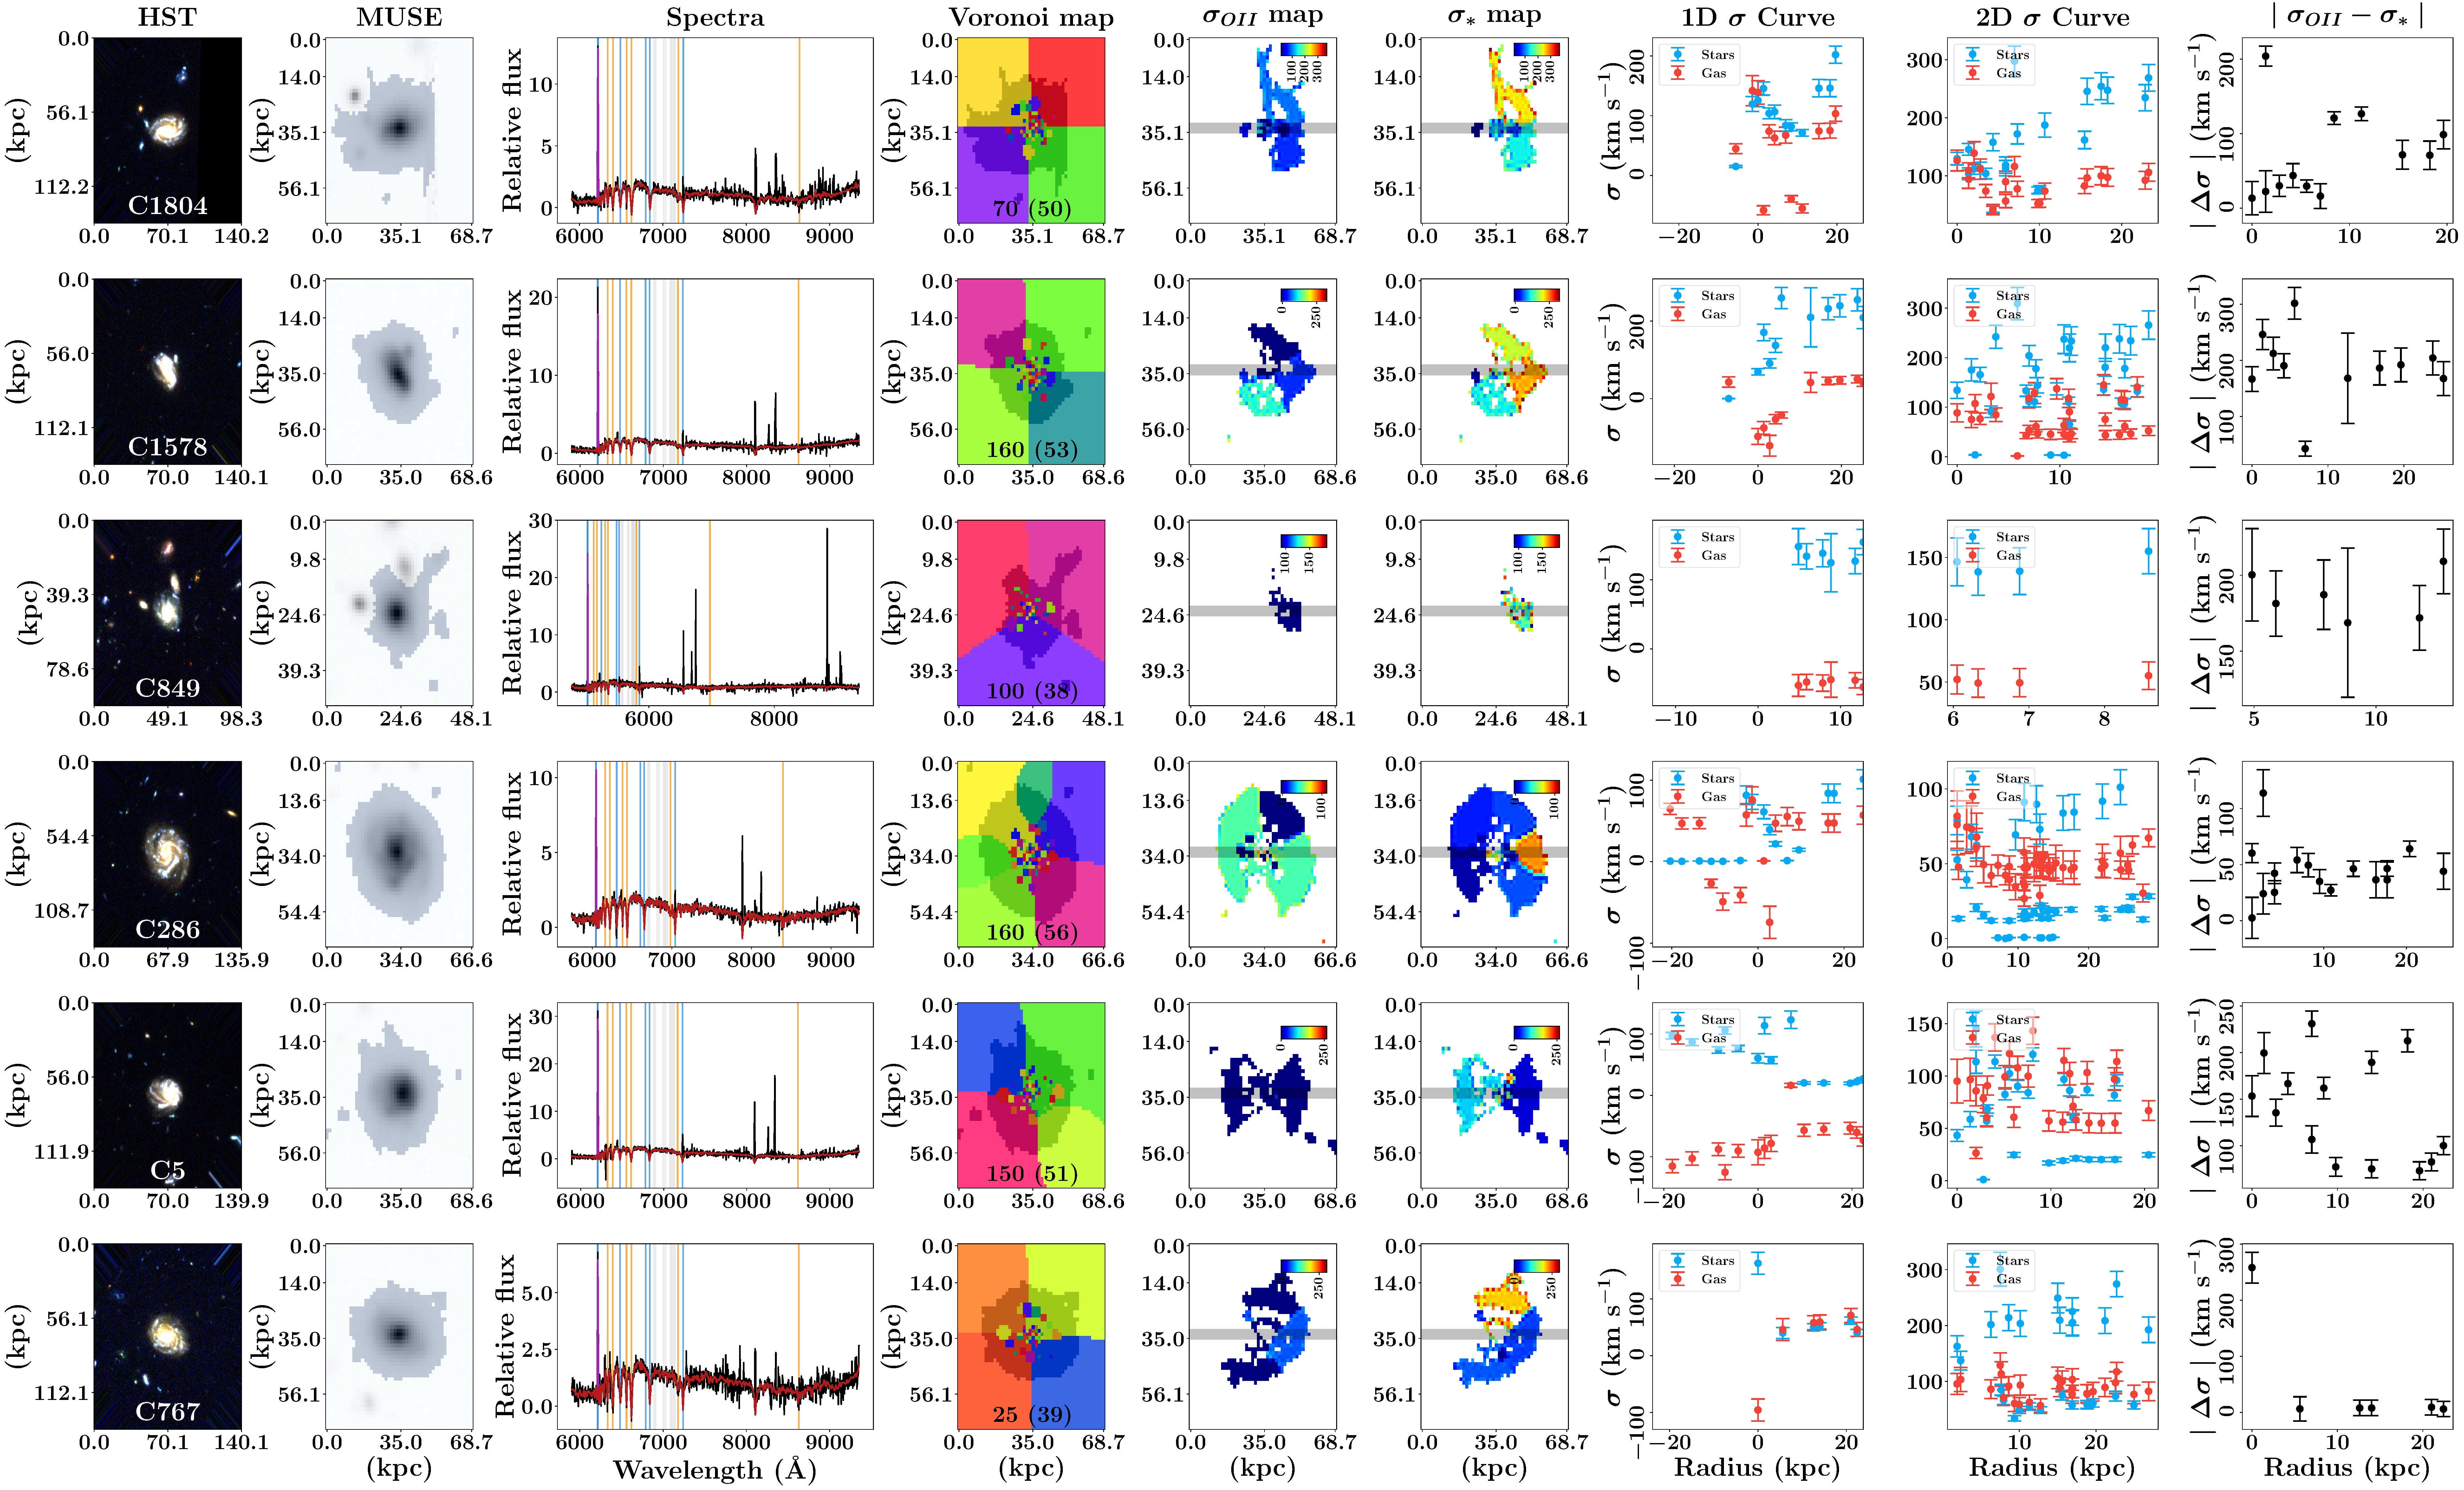
\includegraphics[width=1.0\textheight,height=0.6\textwidth]{data/spectra_complete_velocity_dispersions.pdf}
\caption[Faber--Jackson]{Voronoi tessellation analysis for six galaxies. \textit{HST}: HST image and galaxy cube ID. \textit{MUSE}: collapsed optical image from MUSE spectroscopic data and segmentation map (grey). \textit{Spectra}: galaxy data (black); \texttt{pPXF} model (red); and emission (blue), absorption (orange), and iron (grey) spectral lines. \textit{Voronoi map}: Voronoi tessellated galaxy map and segmentation area. \textit{$\sigma_{OII}$, $\sigma_{*}$ maps}: velocity dispersion $\sigma$ fields. \textit{1D Rot. Curve}: $\sigma$ curve as defined by grey slice across $\sigma$ maps. \textit{2D Rot. Curve}: $\sigma$ curve from galaxy inclination-corrected map. \textit{$\mid V_{OII}-V_* \mid$}: absolute gas and stellar velocity dispersion differences versus galaxy radius with data from 1D $\sigma$ curves.}
\label{fig:multiple_spectra_faber_jackson}
\end{sidewaysfigure}

\end{document}